\chapter{Desarrollo del sistema.}
Para el desarrollo de este sistema espectroscópico se utilizarán los componentes mostrados en la figura \ref{fig:esquema}. A continuación, se explica cómo se utilizó cada uno de los componentes que componen al sistema desarrollado.

\begin{figure}[h]
	\centering
	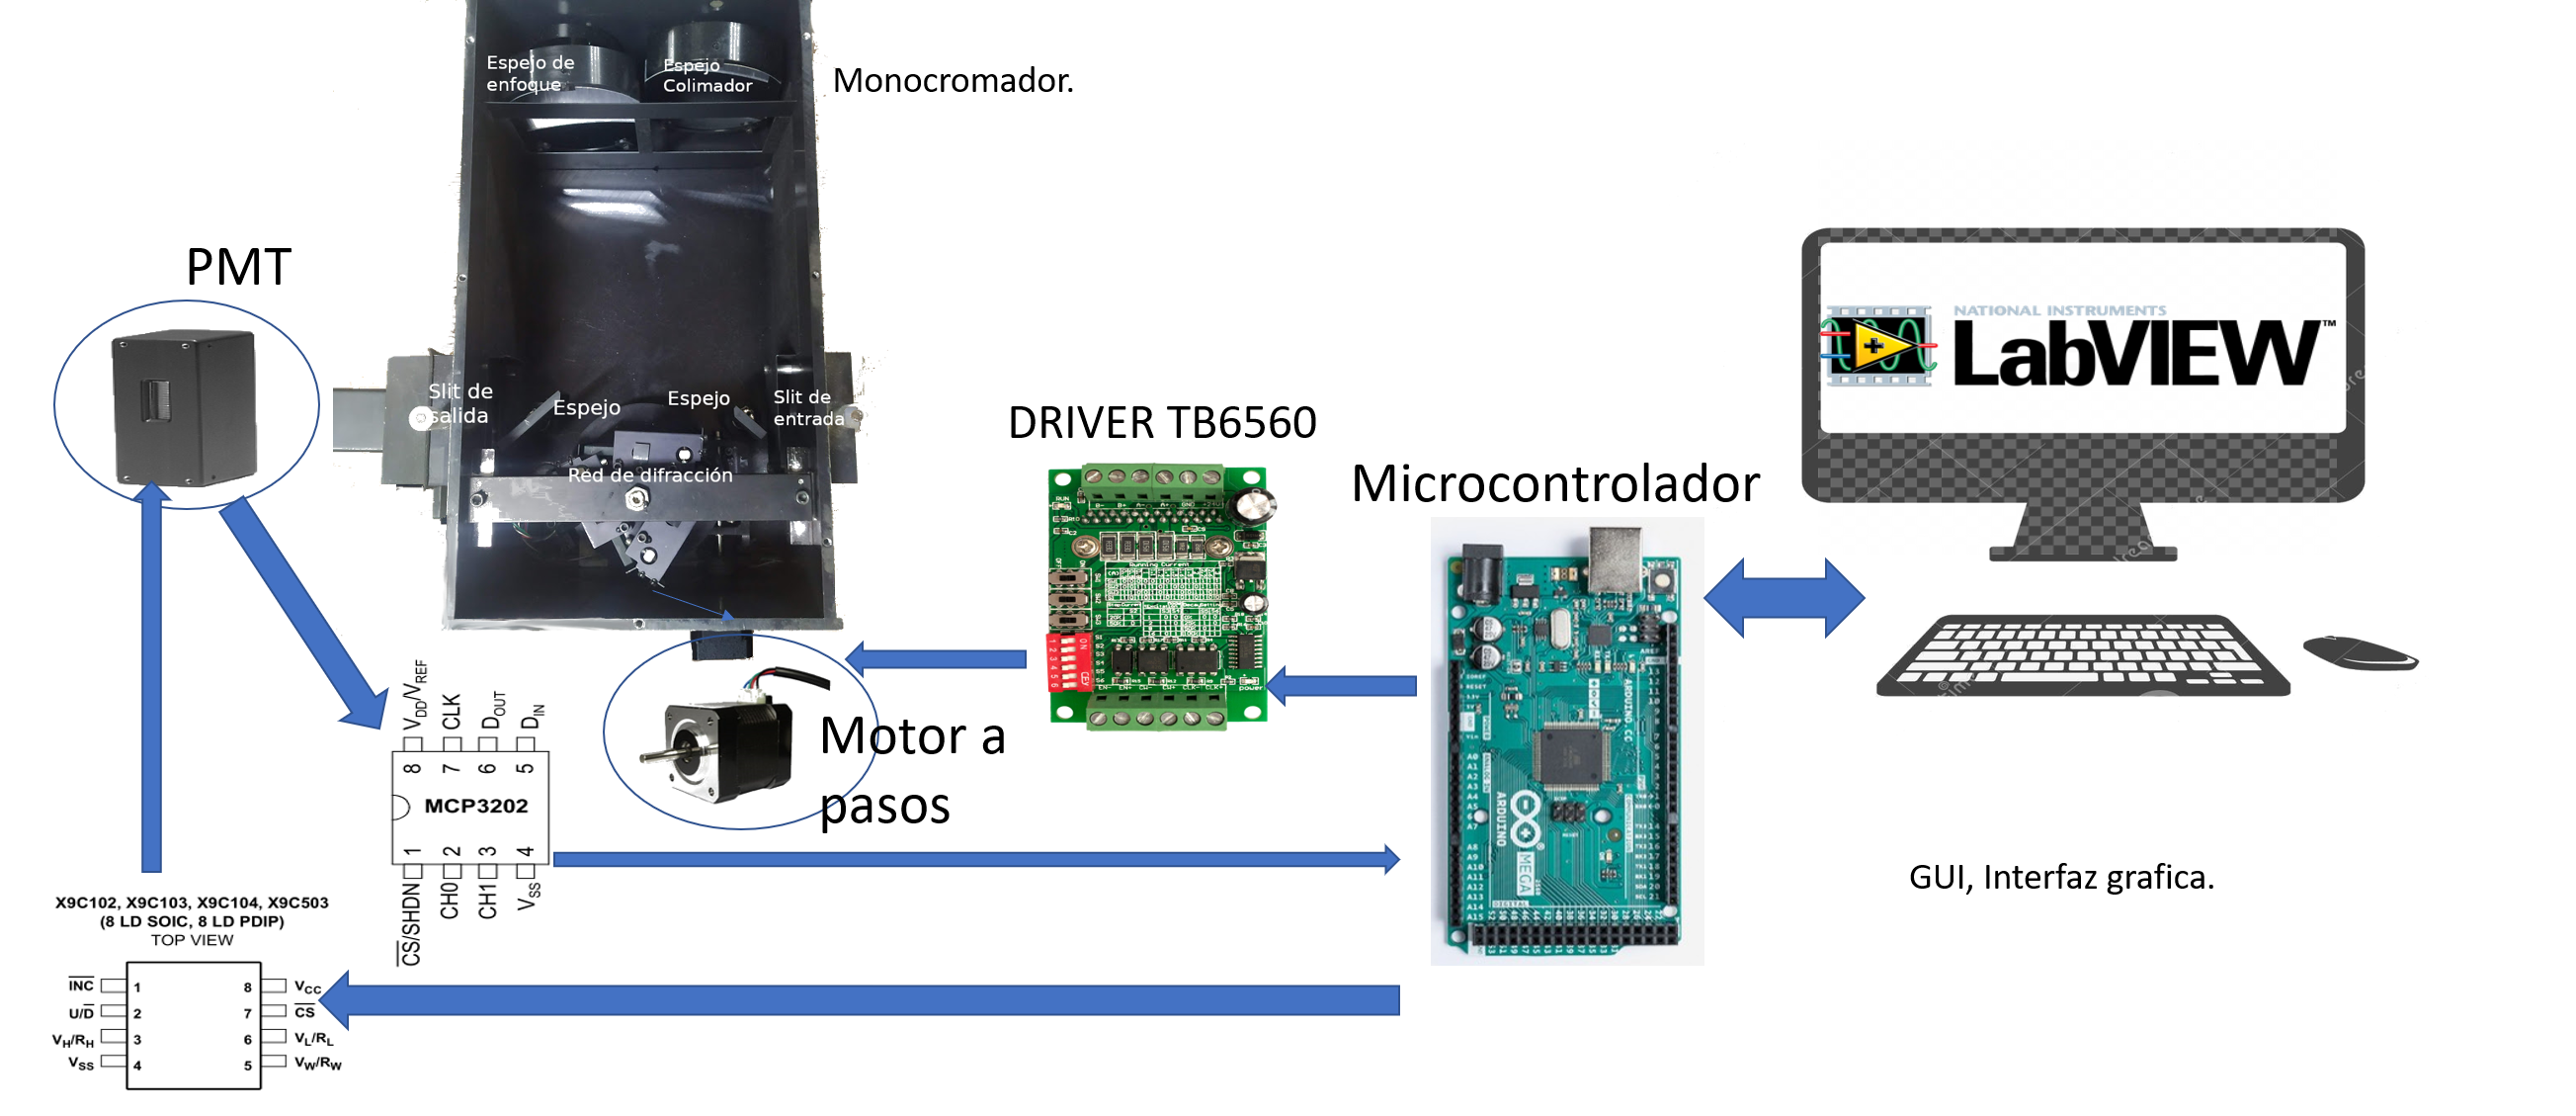
\includegraphics[width=0.98\linewidth]{Imagenes/3/esquema}
	\caption[Esquema donde se muestran los componentes que se usarán para el sistema desarrollado.]{Esquema donde se muestran los componentes que se usan para el sistema desarrollado. El ángulo de la red de difracción dentro del monocromador es modificado por un motor a pasos. El Driver TB6560 controla el motor a pasos. Todo a través de un microcontrolador. La sensibilidad del PMT es cambiada con un potenciómetro digital.}
	\label{fig:esquema}
\end{figure}

\section{Control del monocromador}
El control del monocromador se basa completamente en el control de giro de la red de difracción. Al girar la red se hace un barrido espectral. Este sirve para poder graficar el espectro punto a punto. Desde la parte exterior del monocromador figura \ref{fig:spectrapro}(a) solo se ve el motor a pasos, la apertura, \textit{slit}, para la entrada de la luz a estudiar, y el \textit{slit} de salida, donde se obtiene solo ``una longitud de onda''. El espectrómetro posee la configuración Czerny-Turner, figura \ref{fig:spectrapro}(b), la base que tiene la red de difracción permite colocar tres redes, con lo cual este sistema podría adaptarse a mediciones en otros intervalos del espectro electromagnético, con solo cambiar a una de estas redes. 
\begin{figure}[h]
	\centering
	\subfigure[Monocromador SpectraPro 275]{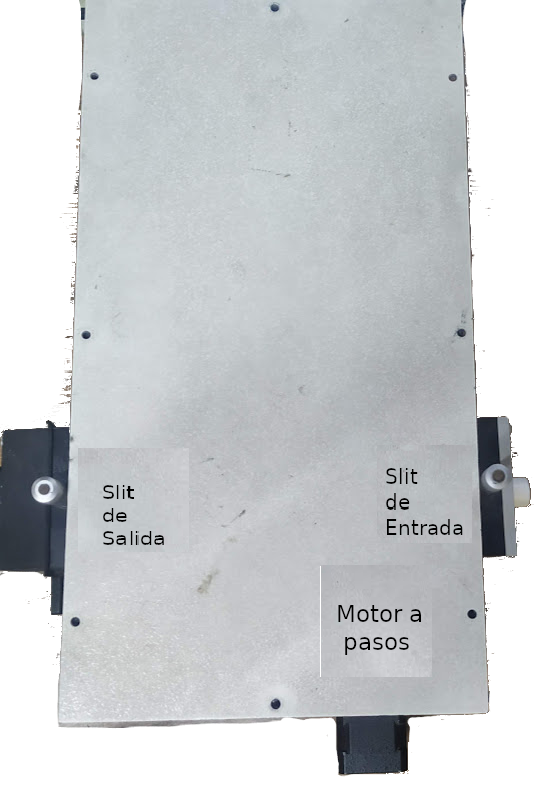
\includegraphics[ height=6cm]{Imagenes/3/SpectraPro}}
	\subfigure[Interior del SpectraPro 275]{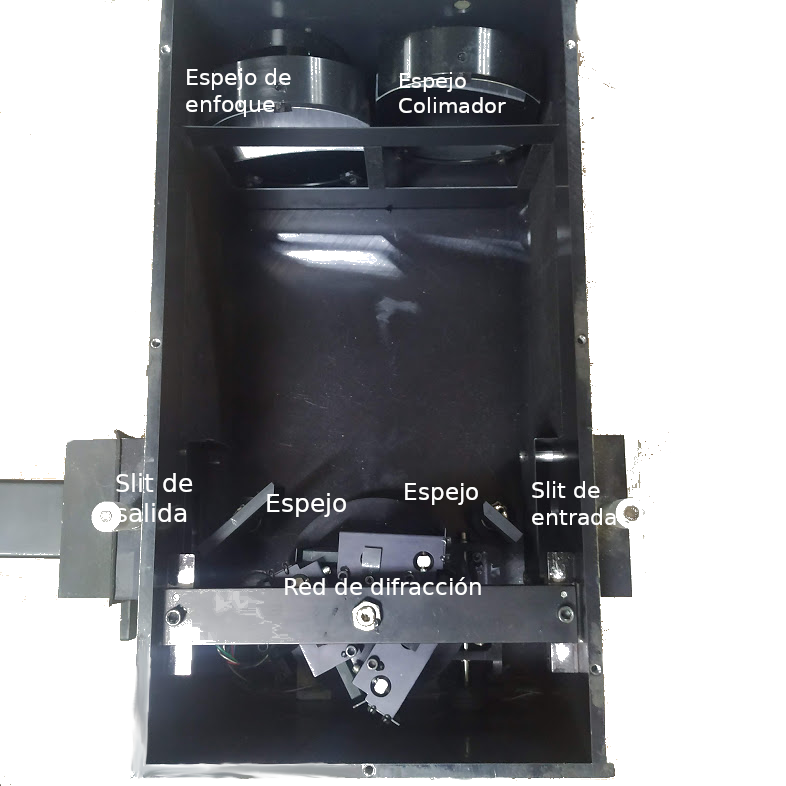
\includegraphics[height=6cm]{Imagenes/3/SpectraProIn}}
	\caption{Monocromador SpectraPro 275 de la compañía Action Research Corporation. Se observa desde una vista superior su exteriror, (izquierda) y su interior (derecha).}
	\label{fig:spectrapro}
\end{figure}

La red de difracción se encuentra montada en una estructura a la cual llamaremos base, está diseñada para poder colocar tres redes de difracción, dentro de la programación del monocromador se tiene la opción de elegir entre estas tres redes, en este proyecto solo se utilizará la red de difracción que tiene mayor densidad de líneas por milímetro, siendo 2400 líneas/mm. En la figura \ref{fig:basered2} se aprecia cómo esta estructura está en el interior del monocromador.
\begin{figure}[h]
	\centering
	\subfigure[Base para tres redes de difracción]{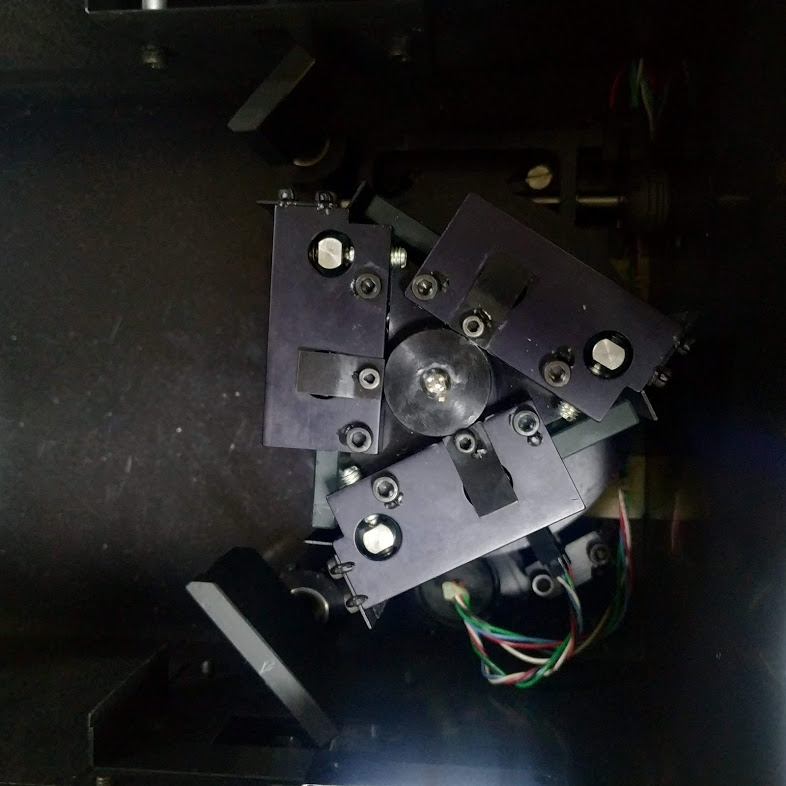
\includegraphics[height=4.5cm]{Imagenes/3/baseRed}}
	\subfigure[Vista frontal de las redes sobre la base.]{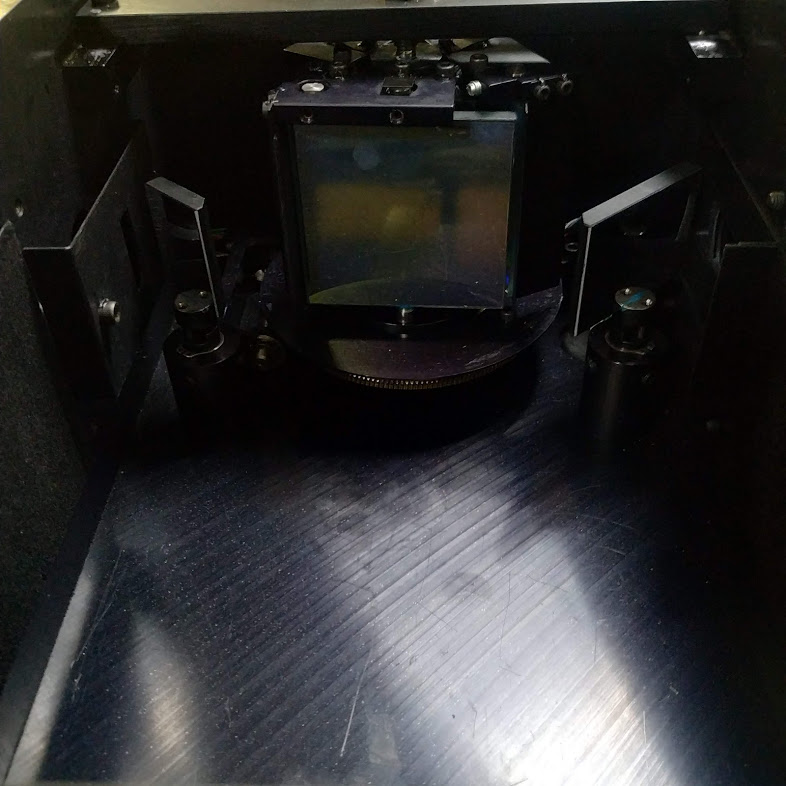
\includegraphics[height=4.5cm]{Imagenes/3/redDifra_in}}
	\caption{Base del monocromador SpectraPro 275, diseñada para colocar 3 diferentes redes de difracción.}
	\label{fig:basered2}
\end{figure}

En la figura \ref{fig:baseredes} se puede ver una rueda dentada, esta rueda junto con un tornillo sin fin, se puede ver en la figura \ref{fig:tornillo}, son los encargados de transmitir el giro del motor a la red de difracción. 
El motor a pasos está conectado al tornillo sin fin, al girar el motor a pasos el tornillo sin fin se desplaza la misma distancia angular $0.9°$ por paso. En la ecuación \ref{equa:tornillo}, $n$ es el número de vueltas, $Z_2$ es la cantidad de dientes en la rueda y $e$ es el número de entradas del tornillo sin fin.  
\begin{equation}
	n_1 e_1 = n_2 Z_2
	\label{equa:tornillo}
\end{equation}
Dado que $e$ siempre será menor que $Z$, este arreglo funciona como un reductor de velocidad.

\begin{figure}[h]
	\centering
	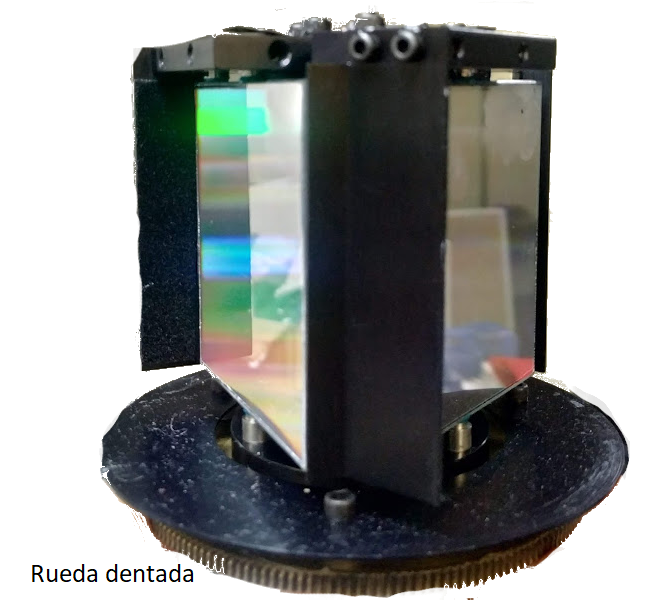
\includegraphics[width=0.4\linewidth,trim={0 0 0 20mm}]{Imagenes/3/baseRedes}
	\caption[Fotografía de la base del monocromador con 3 redes de difracción]{Fotografía de la base, se pueden apreciar dos de las redes de difracción con las cuales cuenta. En la parte inferior se ve la rueda dentada sobre el cual está la base.}
	\label{fig:baseredes}
\end{figure} 
\begin{figure}[h]
	\centering
	\subfigure[Tornillo sin fin]{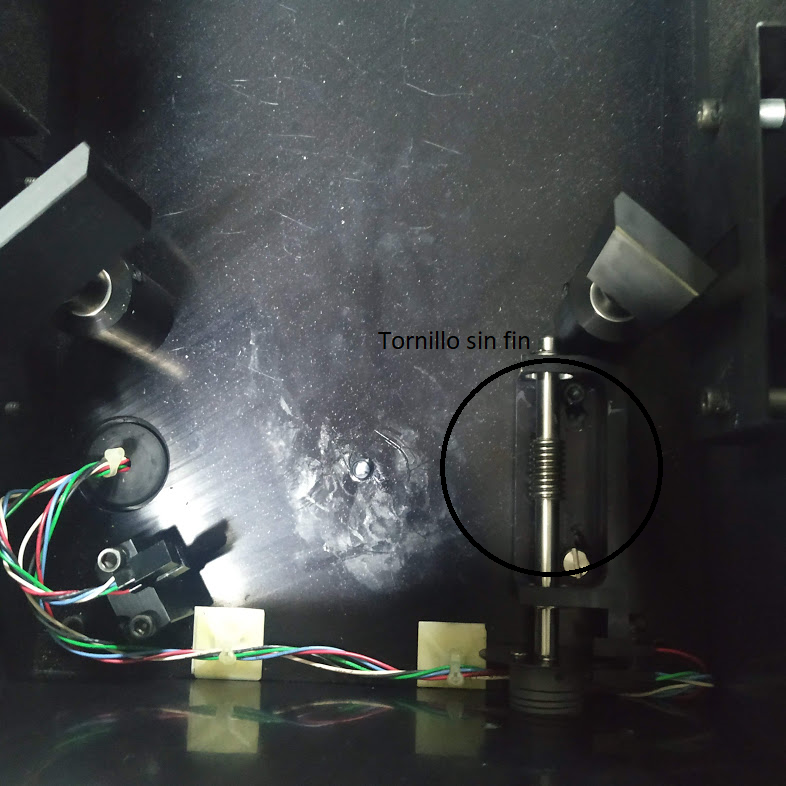
\includegraphics[height=5cm]{Imagenes/3/tornillo}}
	\hspace{10mm}
	\subfigure[base con rueda dentada sobre el tornillo sin fin.]{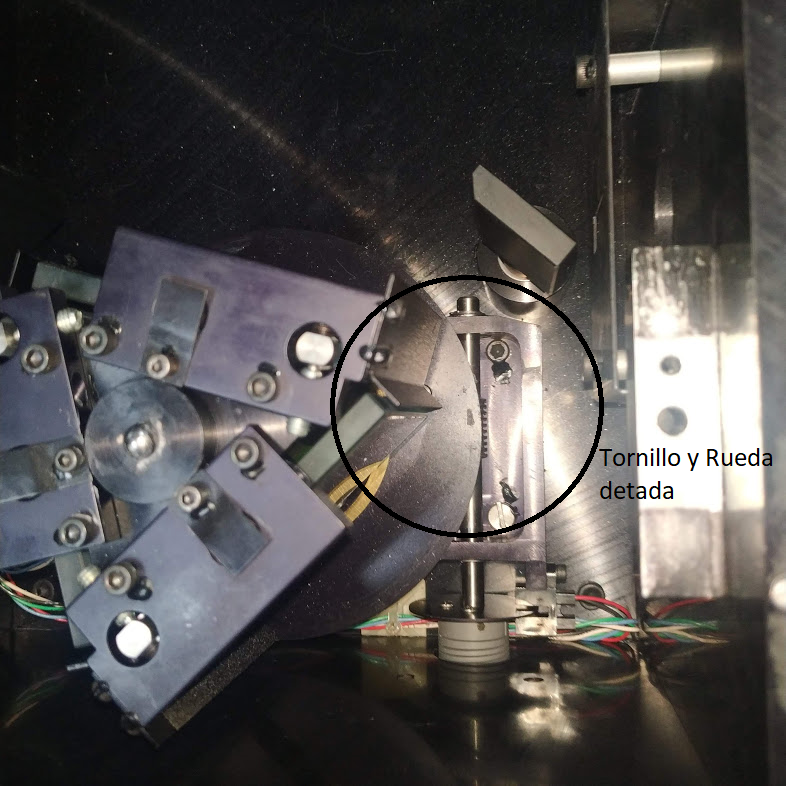
\includegraphics[height=5cm]{Imagenes/3/tornillo_base}}
	\caption{Redes de difracción sobre la base y a su vez sobre el tornillo sin fin.}
	\label{fig:tornillo}
\end{figure}

\section{Control de la red de difracción.}
El control del motor a pasos se realiza con el driver TB6560. Como se mencionó antes solo se necesitan de tres pines para su control. Los cuáles serán los pines 2,3 y 4 del Arduino Mega
\begin{itemize}
	\item pin 2 (dire), se encargará de la dirección del motor.
	\item pin 3 (paso), se encarga del paso del motor, (velocidad, y cantidad de pasos.)
	\item pin 4 (sleep), activa o desactiva el \textit{driver} TB6560
\end{itemize}
%Con un simple algoritmo, donde todos los pines 2, 3 y 4 como salidas. 
El siguiente código hace que el motor a pasos de un solo paso en una dirección (sentido horario). Las variables velL y velH, determinan la velocidad del paso. Si se quiere cambiar el giro del motor solo se debe modificar el valor de \textit{dire} a \textit{LOW}. Ejemplo del código para dar un paso.
\begin{center}
	void pasoMotor() \{ \\
	digitalWrite(sleep, LOW);\\ 
	digitalWrite(dire, HIGH);\\
	digitalWrite(paso, HIGH);\\
	delayMicroseconds(velH);\\
	digitalWrite(paso, LOW);\\
	delayMicroseconds(velL);\\
	\}
\end{center}


%Ya que se puede girar la red de difracción se necesita ubicar a esta en un punto inicial. 
El origen o punto cero, estará determinado por un \textit{encoder}. El monocromador contaba ya con uno, para realizar esta misma función. El \textit{encoder o Optical switch}, es un interruptor óptico. El modelo es el OPB992L51
En la figura \ref{fig:encoder}, se describe el significado de cada uno de las letras y números de este encoder. La información proporciona las características de su empaquetado y como energizar el \textit{encoder}.
\begin{figure}[h]
	\centering
	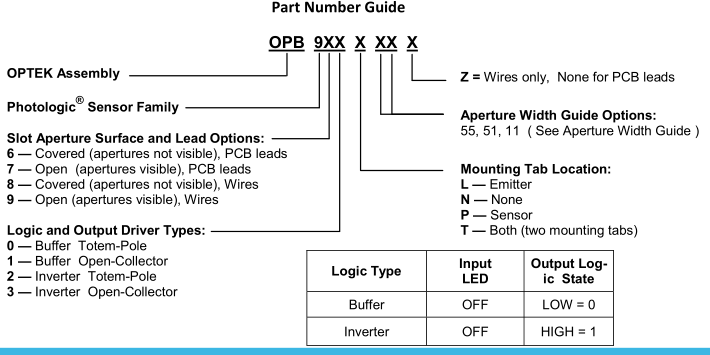
\includegraphics[width=0.8\linewidth]{Imagenes/3/Encoder}
	\caption{Información del \textit{encoder}, la nomenclatura de este indica su funcionamiento \cite{OPB992}}
	\label{fig:encoder}
\end{figure}
El encoder es el OPB992L51 lo que significa:
\begin{itemize}
	\item OPB, OPTEK Assebly
	\item 9, Familia de sensores \textit{Photologic}
	\item 2 \textit{Inverter Totem-Pole} ver figura \ref{fig:OPB}
	\item L \textit{Emitter}, figura \ref{fig:emitter} (a) y (b).
	\item 51 tamaño de la apertura \ref{fig:emitter} (c).
\end{itemize}
Para poner en funcionamiento el \textit{encoder} solo se tiene que energizar el diodo emisor con los cables rojo y negro, el cable negro va al GND del Arduino, al igual que el cable verde. En la figura \ref{fig:OPB} se observa el cableado del \textit{encoder}. El cable rojo va al Arduino a un PIN de salida, PIN 13, que solo se pone en alto cuando se va a usar el \textit{encoder}, mientras busca la posición cero. El cable azul dará la respuesta cuando su valor esté en bajo significará que se ha encontrado la posición cero, se leerá con el PIN 12 del Arduino.

\begin{figure}[h]
	\centering
	\subfigure[diagrama del encoder.]{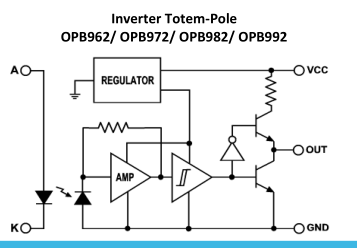
\includegraphics[height=40mm]{Imagenes/3/Inverter}}
	\subfigure[Color de los cables]{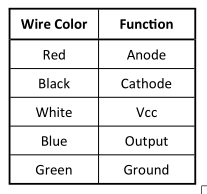
\includegraphics[height=40mm]{Imagenes/3/Cables}}
	\caption{Información del cableado del \textit{encoder}\cite{OPB992}}
	\label{fig:OPB}
	
\end{figure}
\begin{figure}[h]
	\centering
	\subfigure[]{	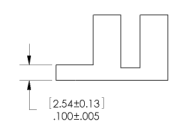
\includegraphics[height=30mm]{Imagenes/3/Emitter}}
	\subfigure[]{	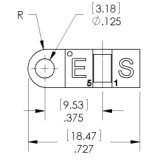
\includegraphics[height=30mm]{Imagenes/3/Emitter2}}
	\subfigure[Dimensión de apertura del encoder]{	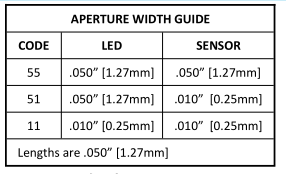
\includegraphics[height=30mm]{Imagenes/3/51}}
	\caption{Dimensiones del encoder. \cite{OPB992}}
	\label{fig:emitter}
\end{figure}
\begin{figure}[h]
	\centering
	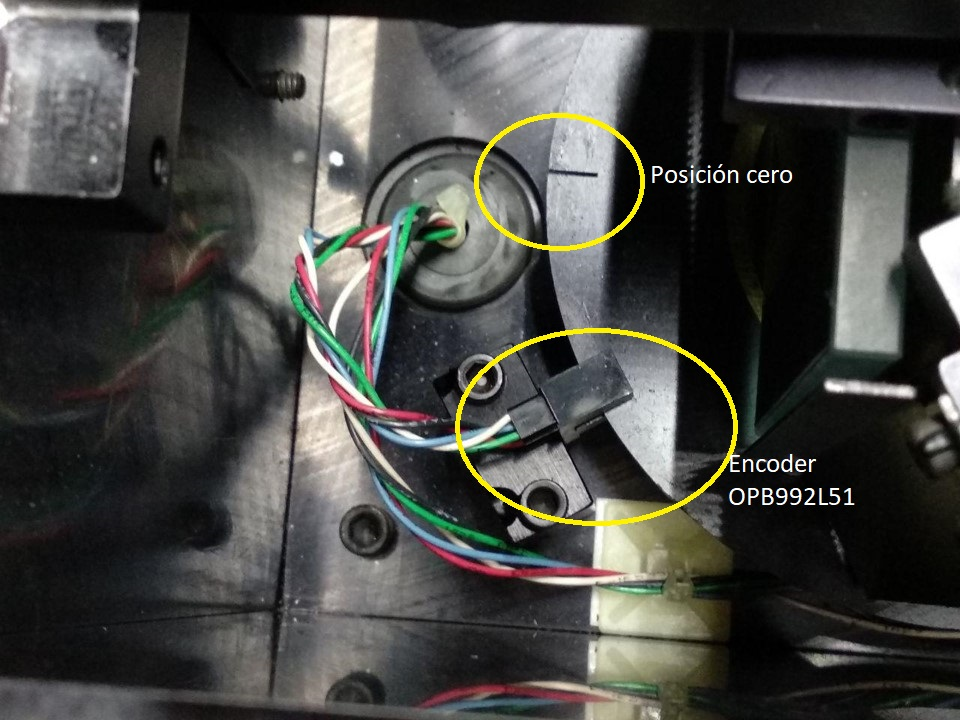
\includegraphics[width=0.7\linewidth,height= 7cm]{Imagenes/3/Encoder_01}
	\caption{Posición cero del sistema, el motor gira hasta que el \textit{encoder} encuentre la ranura de la posición cero.}
	\label{fig:encoder01}
\end{figure}

Al iniciar la búsqueda de la posición cero,
se activa el \textit{encoder} y se hace girar el motor en una dirección de forma continua. El motor hará girar la red de difracción. Al encontrar la posición cero, véase figura \ref{fig:encoder01}. el motor avanzará 400 pasos en la dirección opuesta y regresará a buscar la posición cero, para garantizar que realmente sí la encontró.
Con este algoritmo se coloca el motor en su posición inicial. Para activar el motor se usa una interfaz gráfica en la cual se realiza esta acción con botón 1 de la figura \ref{fig:GUI_01} (1). Al presionar \textbf{INICIAR}, se manda una instrucción al Arduino de girar el motor hasta encontrar la posición inicial, el motor girará mientras en el PIN 12 tenga un valor en ``ALTO'' (5V), cuando el valor este en bajo (0V), el motor estará en su posición inicial.

\begin{figure}[h]
	\centering
	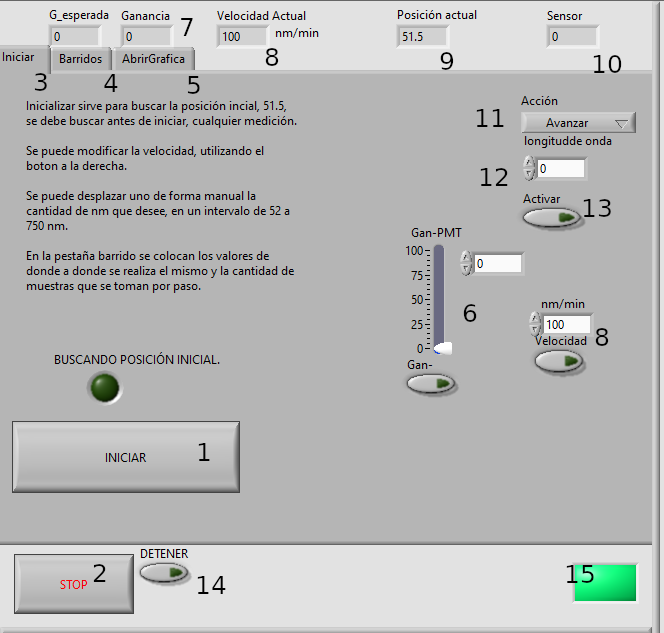
\includegraphics[width=0.8\linewidth]{Imagenes/3/GUI_01}
	\caption{Interfaz gráfica diseñada para inicializar el sistema.}
	\label{fig:GUI_01}
\end{figure}

\section{Calibración.}
\subsection{Lámpara de mercurio.}
Lo siguiente es realizar los barridos en el intervalo del espectro electromagnético. A partir de la posición cero el motor se movería paso a paso, donde se tendrá el registro de cada paso. El motor hará girar la red de difracción, desde los 0 pasos hasta los 10000 pasos. Con el algoritmo desarrollado se puede determinar cuantos pasos dar, y en qué sentido. Utilizando el \textit{PMT}, obtendremos un valor de voltaje, proporcional a la intensidad de luz. Se tendrá una gráfica pasos vs. voltaje(bits). 
Para esta medición el motor dará un paso, se tomará un valor del \textit{PMT} con el ADC del Arduino MEGA, que tiene una resolución de 10 bits. La información del paso y valor será enviado a la interfaz gráfica, para obtener un espectro que se irá formando paso a paso. En la figura \ref{fig:ledqe65} se aprecia la forma del espectro del led amarillo utilizando nuestro sistema. 


Al comparar los espectros obtenidos, figura \ref{fig:ledqe65}, por nuestro sistema y el espectrómetro QE65000. Se aprecia un espectro mejor definido en el QE65000. Para mejorar el espectro medido por nuestro sistema, se realiza la toma de más muestras por paso, y se obtiene un promedio en cada punto. Con un máximo de 99 muestras por paso, ver figura \ref{fig:led99muestras}.
\begin{figure}[h]
	\centering
	\subfigure[Sistema propuesto.]{	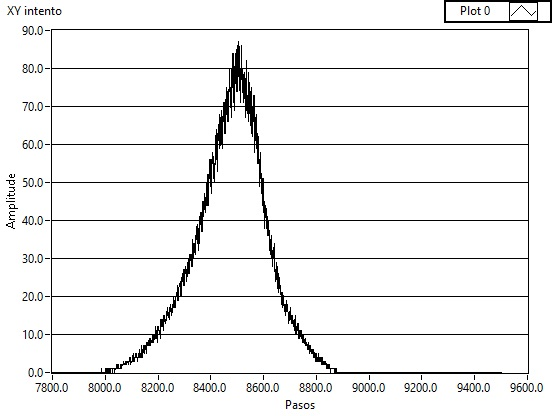
\includegraphics[width=0.45\linewidth]{Imagenes/3/10s30khz-02}}
	\subfigure[QE65000]{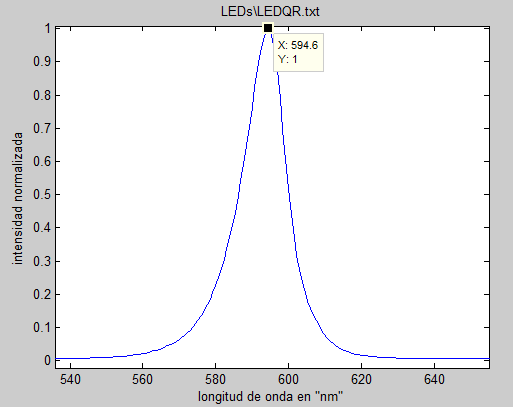
\includegraphics[width=0.45\linewidth]{Imagenes/3/LEDQE65}}
	\caption{Espectro del LED amarillo medidos con el sistema propuesto (a) y con el QE65000 (b).}
	\label{fig:ledqe65}
\end{figure}

\begin{figure}[h]
	\centering
	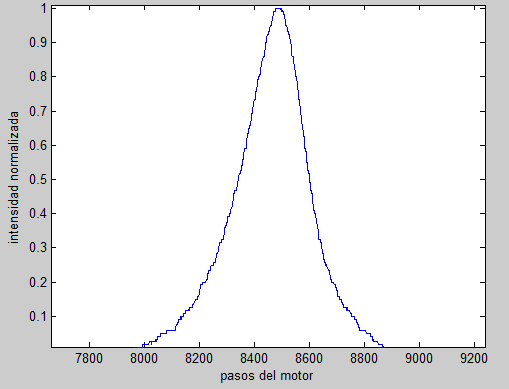
\includegraphics[width=0.9\linewidth,height=6cm]{Imagenes/3/LED99Muestras}
	\caption[Espectro de un LED amarillo.]{Captura del espectro de un LED amarillo, tomando 99 muestras por punto.}
	\label{fig:led99muestras}
\end{figure}
La cantidad de muestras que se toma por punto es de suma importancia para obtener un espectro más limpio y sin tantas variaciones punto a punto.
Para la calibración del sistema utilizaremos 99 muestras por paso para poder medir el espectro de la lámpara de mercurio. Esto con el fin de adquirir un espectro lo más limpio posible y poder obtener la relación paso a longitud de onda. Las líneas de emisión de la lámpara de mercurio a buscar son 12. En la figura \ref{fig:mercuriolineas} se en listan.
\begin{figure}[h]
	\centering
	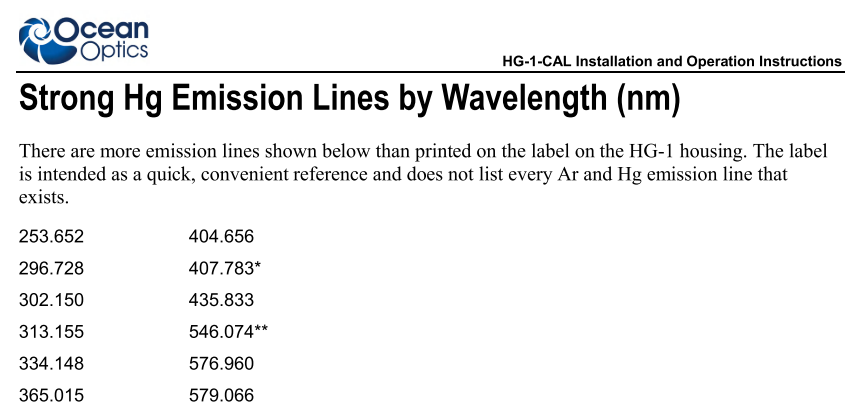
\includegraphics[width=0.8\linewidth,height=5cm]{Imagenes/3/Mercuriolineas}
	\caption{Líneas de emisión de la lámpara de Mercurio. Lámpara de Ocean Optics HG-1 Mercury Argón. \cite{Excel2000}}
	\label{fig:mercuriolineas}
\end{figure}

En la figura \ref{fig:hg-04-m99-50pps}, se pueden apreciar 11 líneas de forma fácil más una de ellas es un segundo orden de la primera longitud de onda de mayor intensidad de la lámpara de mercurio ($\lambda_{253}$ línea (1), su segundo orden $\lambda_{507}$ (8)). Esto se demuestra más adelante utilizando un filtro pasa alto mayor a 400nm. Entre las líneas 2 y 4 se alcanza a visualizar una tercera línea, figura \ref{fig:hg-04-m99-50pps} . Entre las líneas 1 y 2 se observa otra pequeña línea (x) de la lámpara. Primero identificaremos las líneas de emisión principales de la lámpara de mercurio en nuestro espectro. Estas líneas facilitan la obtención de la relación paso longitud de onda.

\begin{figure}[h]
	\centering
	\subfigure[Espectro de la lámpara de mercurio HG-01 de Ocean Optics]{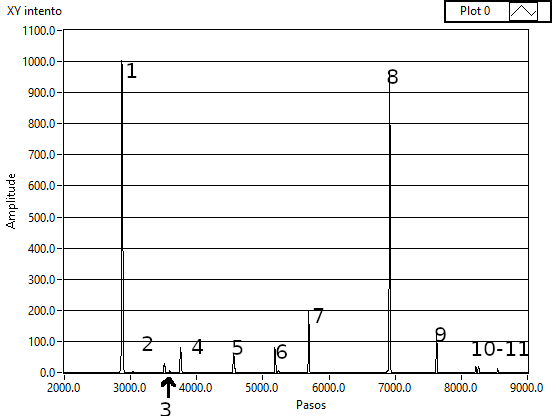
\includegraphics[width=0.48\linewidth,height=50mm]{Imagenes/3/Hg-04-m99-50pps}}
	\subfigure[Acercamiento a las líneas de emisión.]{	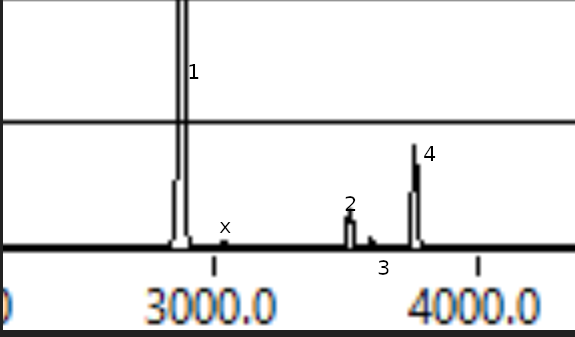
\includegraphics[width=0.48\linewidth,height=45mm]{Imagenes/3/mercuriozoom}}
	
	\caption{Espectro medido con el sistema desarrollado, intensidad contra pasos del motor.}
	\label{fig:hg-04-m99-50pps}
\end{figure}

La lámpara de mercurio tiene en realidad más de 12 líneas de emisión, véase figura \ref{fig:emisionhglibro}. Para poder observarlas se requieren de sistemas de alta resolución y sensibilidad \cite{CRC2016}. Para calibrar el sistema se utilizaron 12 líneas de emisión, ver figura \ref{fig:mercuriolineas}.
% En el libro de \textit{CRC Handbook of Chemistry and Physics"}podemos ver todas las líneas de emisión del mercurio, la figura \ref{fig:espectromercurio}, es una tabla sacada de este libro donde se ven las intensidades y las longitudes de onda (en ángstrom \r{A}) del espectro de emisión de la lámpara de mercurio. En números romanos se encuentra el grado de ionización del mercurio, para nosotros es solo (I) el de interés. Esta es la razón de que en el espectro aparezcan más de las líneas de emisión. 
\begin{figure}
	\centering
	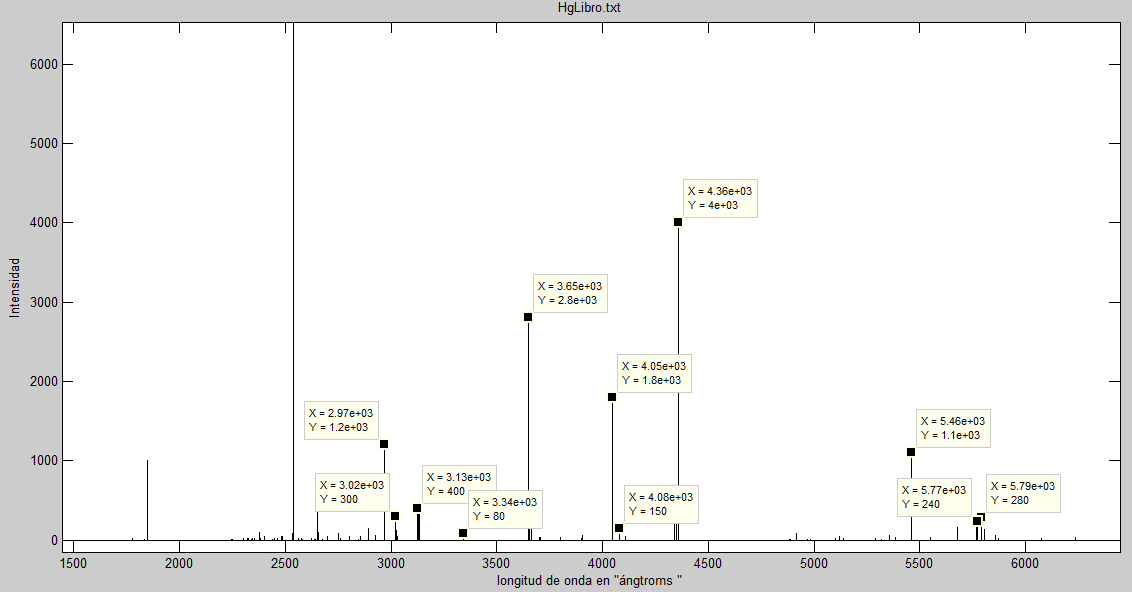
\includegraphics[width=0.9\linewidth,height=5cm]{Imagenes/3/emisionHgLibro}
	\caption{Espectro de emisión del mercurio, se aprecian más de 12 líneas de emisión. Se resaltan las 12 líneas que usaremos para calibrar el sistema desarrollado, \cite{CRC2016}.}
	\label{fig:emisionhglibro}
\end{figure}


\subsection{Relación pasos a longitud de onda.}

Se identificaron los  máximos de cada pico dentro de la medición del espectro adquirido por el sistema. Con los datos obtenidos se graficó el espectro utilizando MATLAB, ver figura \ref{fig:ms1-r}(a). Al hacer un acercamiento al espectro de las líneas de emisión, se logran visualizar más líneas, véase figura \ref{fig:ms1-r}(b). 

%\begin{figure}
%	\centering
%	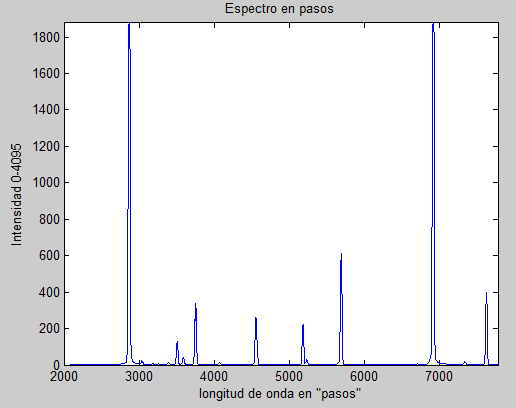
\includegraphics[width=0.7\linewidth,height=4cm]{Imagenes/3/ms1}
%	\caption{Espectro de la lámpara de mercurio}
%	\label{fig:ms1}
%\end{figure}


\begin{figure}[h]
	\centering
	\subfigure[Pondremos atención a ese recuadro.]{	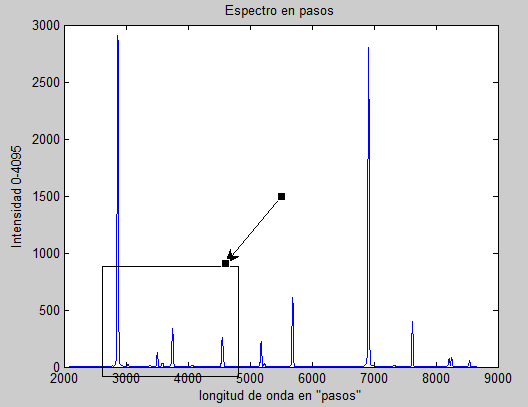
\includegraphics[width=0.45\linewidth,height=3.5cm]{Imagenes/3/ms1-r}}
	\subfigure[Se observan más líneas de emisión]{	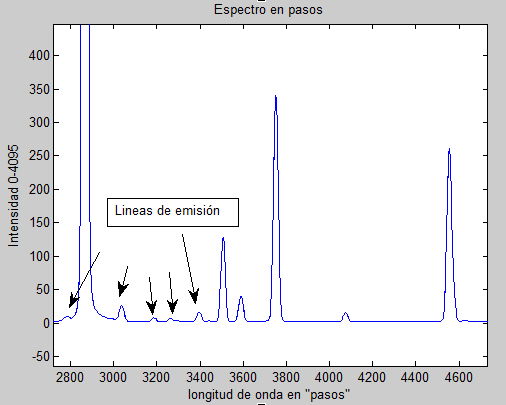
\includegraphics[width=0.45\linewidth,height=3.5cm]{Imagenes/3/ms1-z}}
	\caption{Líneas de emisión del mercurio. Obtenidas por el sistema, su relación es en pasos y no en longitud de onda.)}
	\label{fig:ms1-r}
\end{figure}


%colocar aquí la imagen faltante.

%\newpage

%\begin{figure}[h]!
%	\centering
%	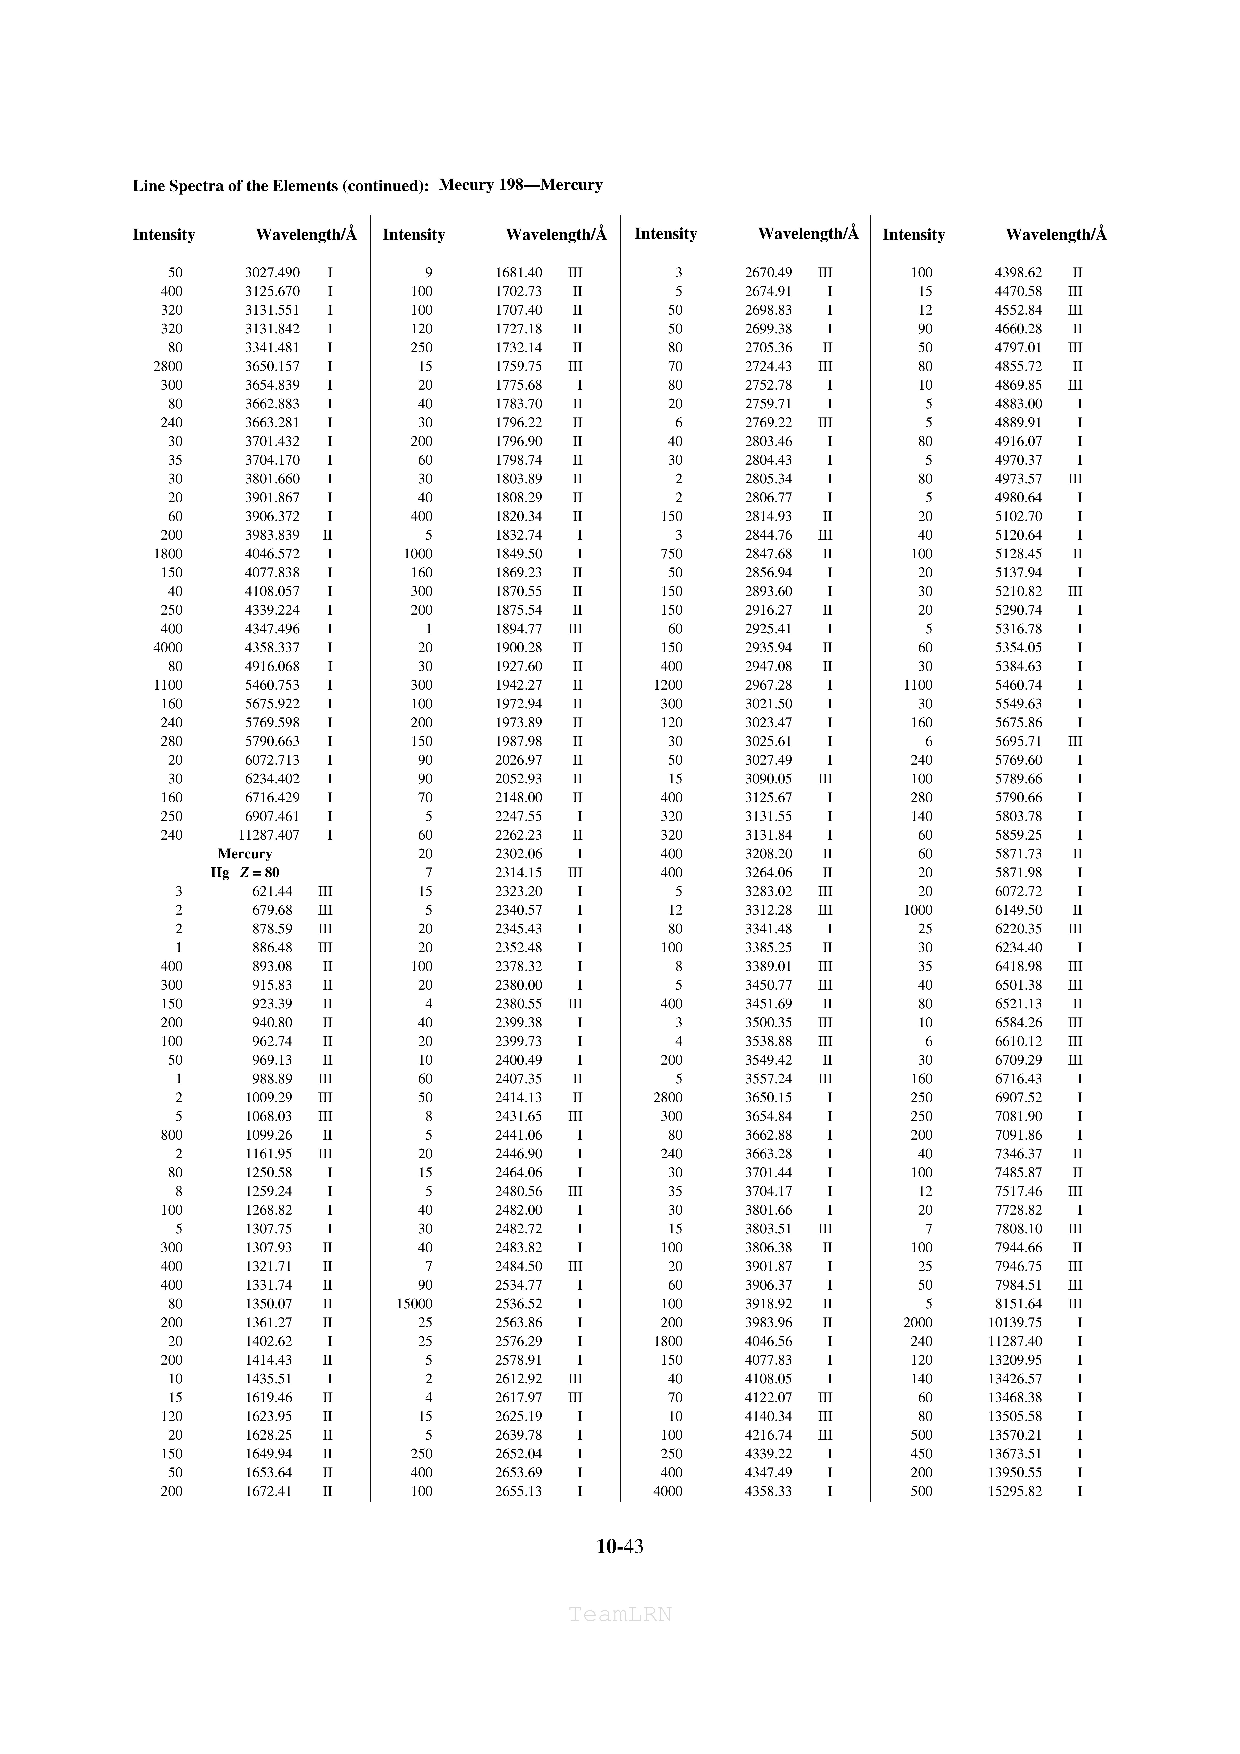
\includegraphics[width=1\linewidth]{Imagenes/3/EspectroMercurio}
%	\caption{Espectro del mercurio, en números romanos esta el grado de ionización. \cite{Water2017}}
%	\label{fig:espectromercurio}
%\end{figure}

Se realizaron 10 mediciones del espectro de la lámpara de mercurio. En cada una se regresó al punto inicial, posición cero. 

%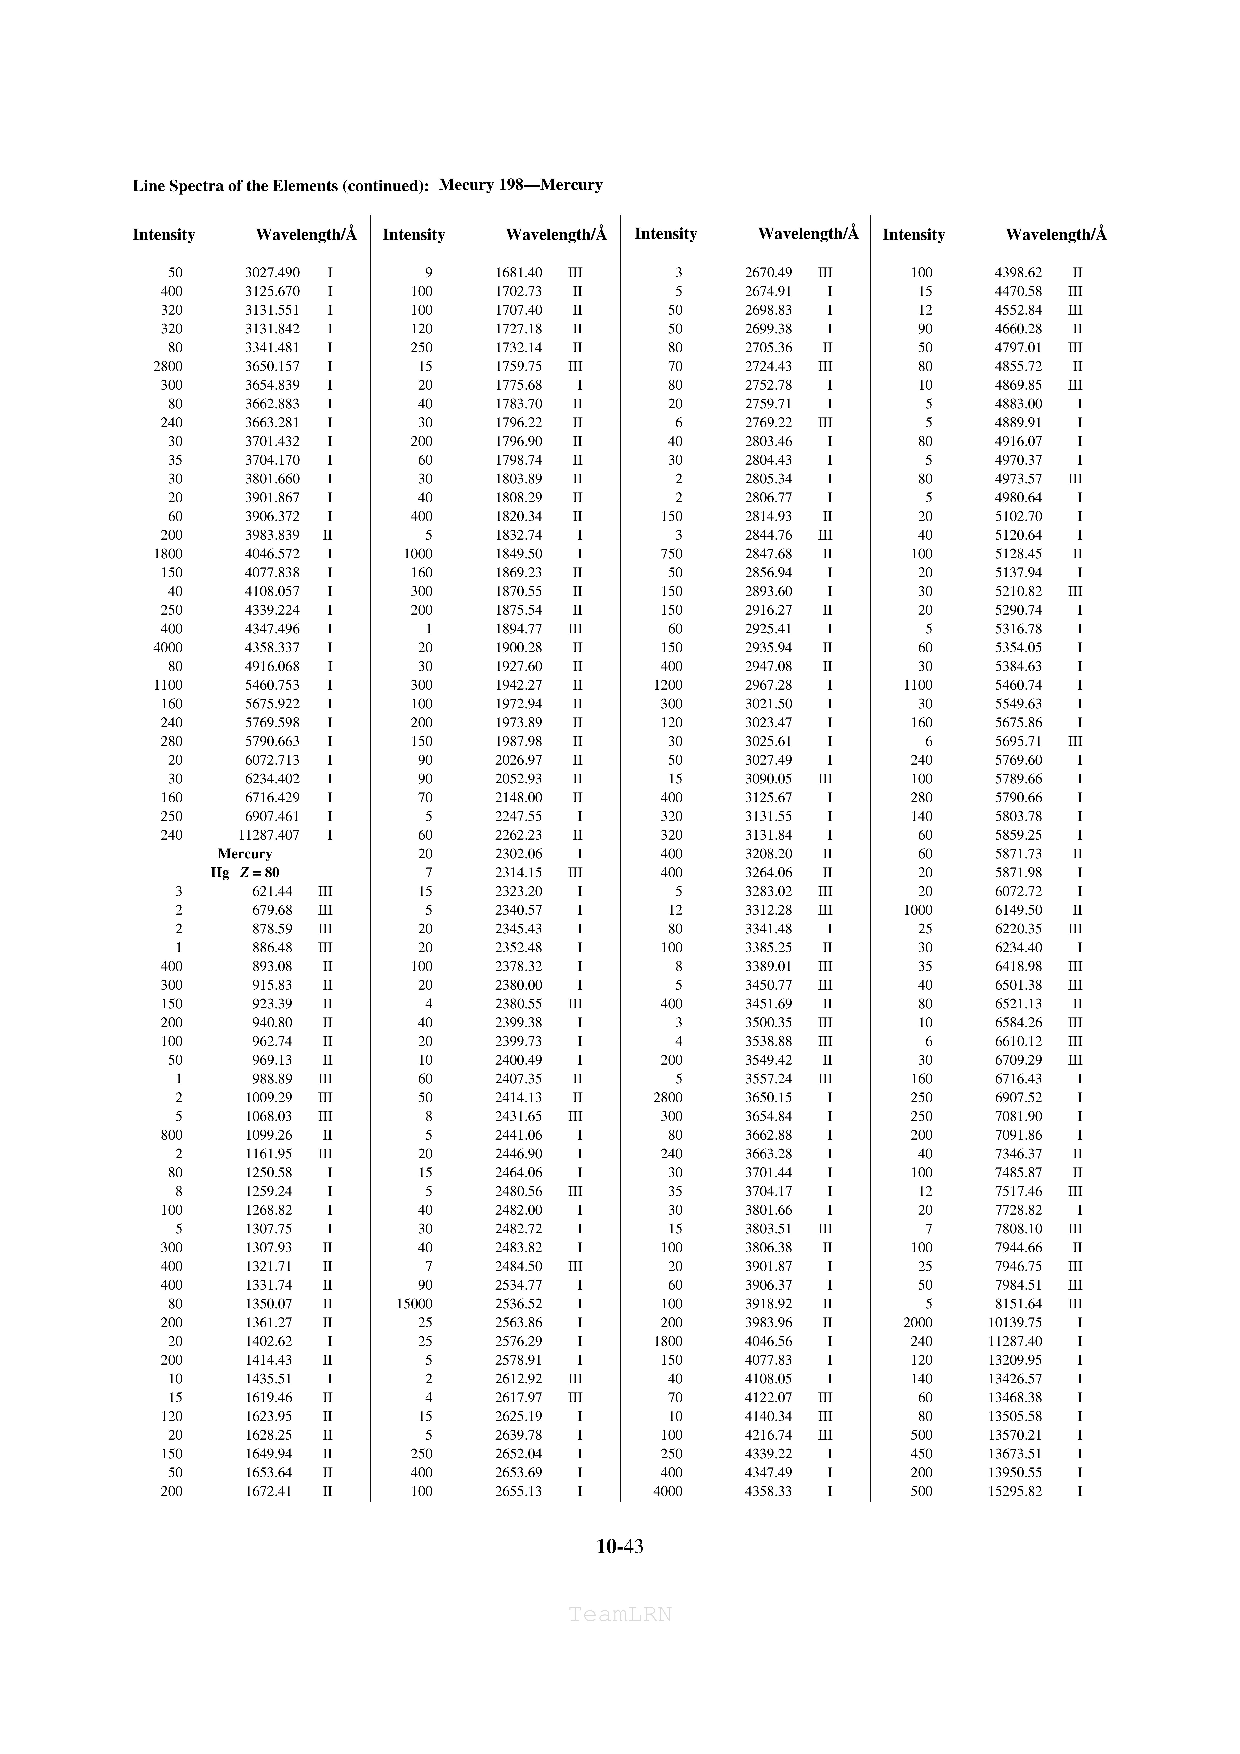
\includepdf[pages={1},scale=1,pagecommand={}]{Imagenes/3/EspectroMercurio.pdf}

En la figura \ref{fig:medi1}(a) se grafica un solo espectro. Al graficar 10 mediciones del mismo espectro para ver la repetitividad del sistema, véase figura \ref{fig:medi1}(b) se aprecia que hay pocas variaciones entre cada medición. En la figura \ref{fig:medi1}(c), se ve solo uno de los picos de emisión. Cada medición del espectro entrega las mismas líneas de emisión. 

\begin{figure}[h]
	\centering
	\subfigure[Espectro de la lámpara de mercurio medido.]{	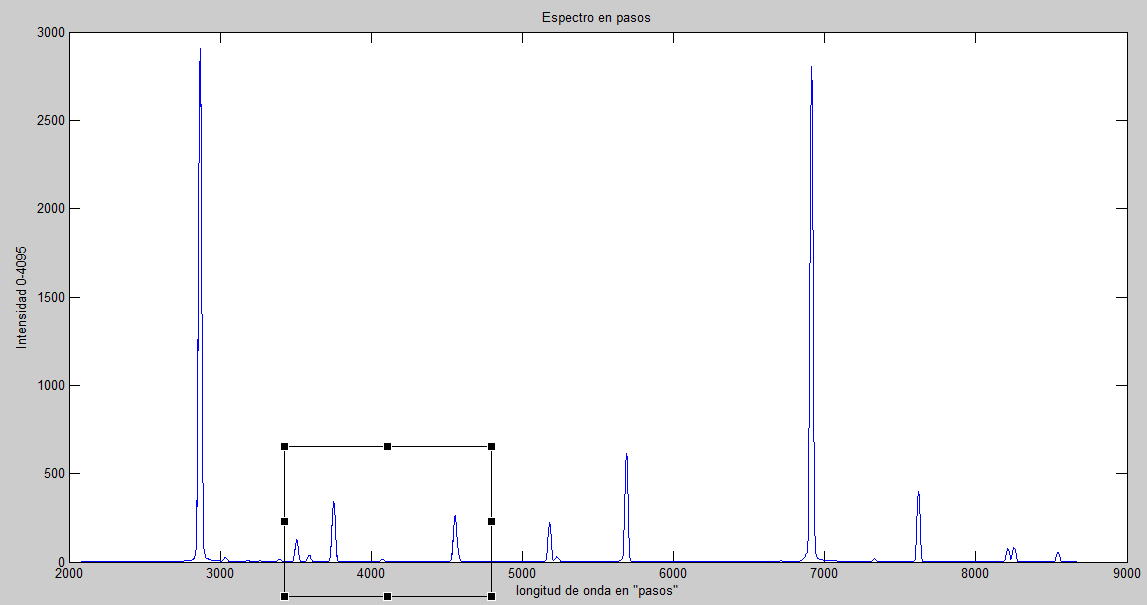
\includegraphics[width=0.4\linewidth, height=3cm]{Imagenes/3/medi1}}
	%\subfigure[nos enfocamos en una intervalo.]{	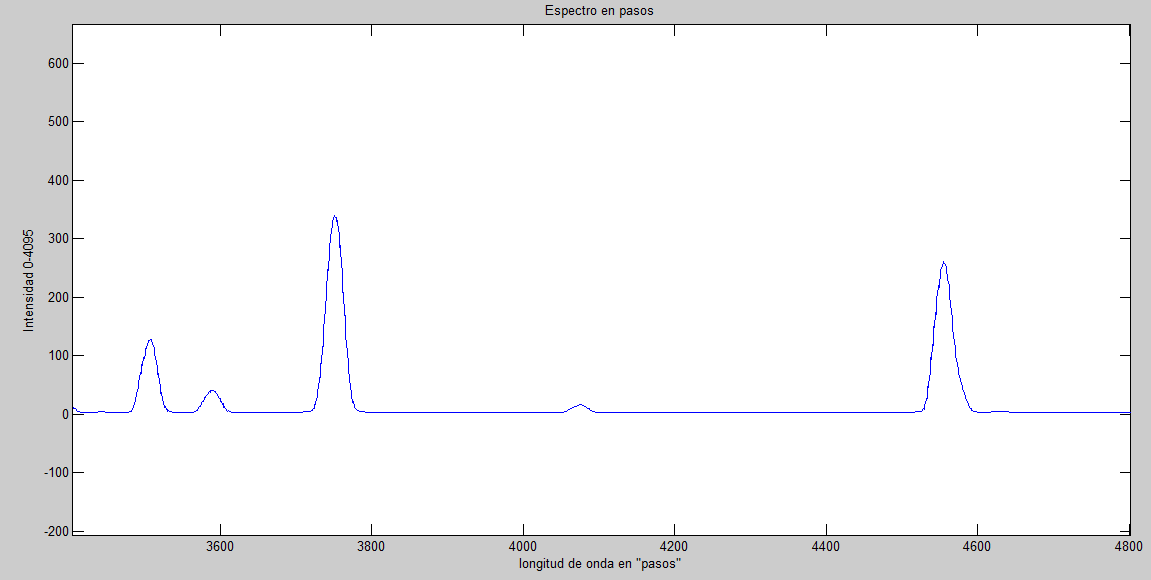
\includegraphics[width=0.4\linewidth]{Imagenes/3/medi1-z}}
	%\subfigure[10 mediciones juntas.]{	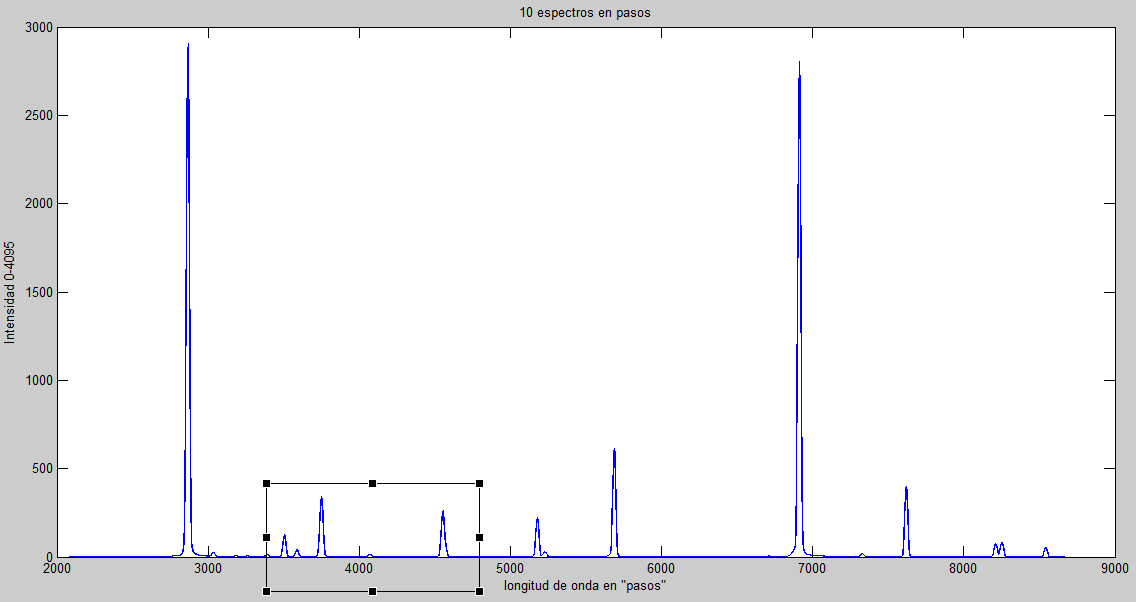
\includegraphics[width=0.4\linewidth]{Imagenes/3/medi10}}
	\subfigure[gráfica con 10 mediciones del espectro de la lámpara de mercurio.]{	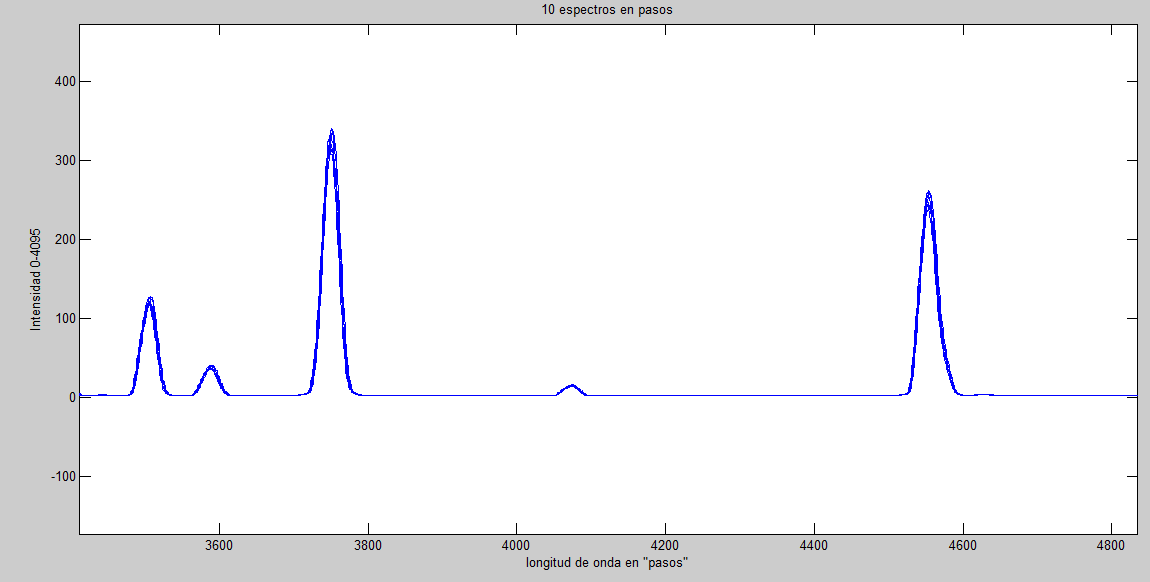
\includegraphics[width=0.4\linewidth, height=3cm]{Imagenes/3/medi10-z}}
	%\subfigure[aún más cerca en la medición.]{	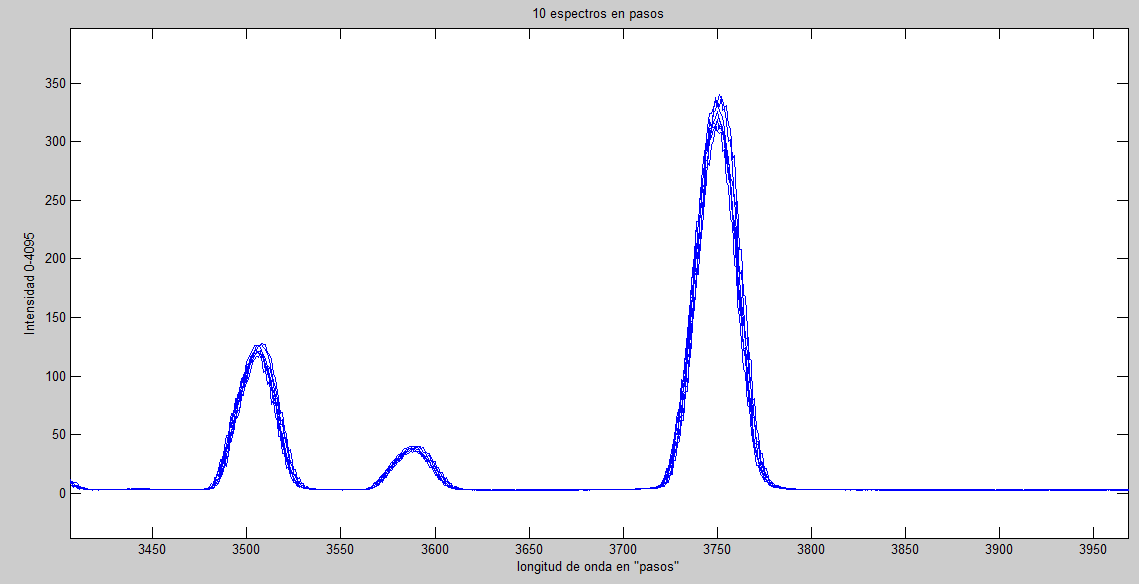
\includegraphics[width=0.4\linewidth]{Imagenes/3/medi10-z2}}
	\subfigure[Se observa la repetitividad a la hora de medir del sistema, nos enfocamos en solo un pico.]{	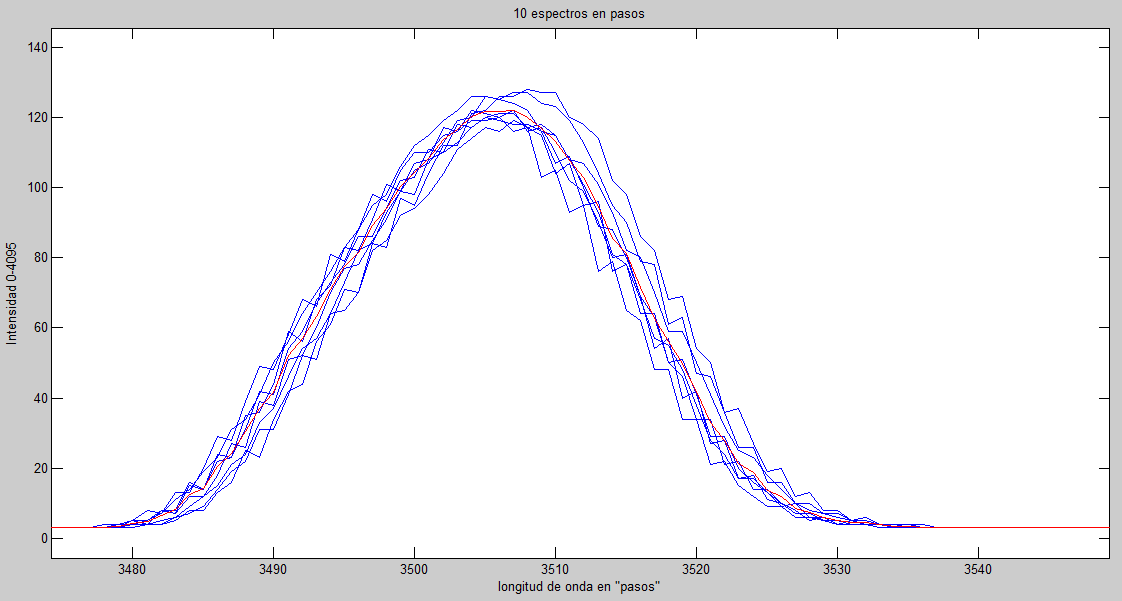
\includegraphics[width=0.7\linewidth, height=3cm]{Imagenes/3/medi10-p}}
	
	\caption[Espectro de la lámpara de mercurio. Se aprecia la repetitividad del sistema.]{Espectro de la lámpara de mercurio. se grafican varias mediciones de este espectro para poder observar la repetitividad del sistema a la hora de obtener espectros.}
	\label{fig:medi1}
\end{figure}
Se usan estas mediciones del espectro de la lámpara de mercurio para encontrar las 12 líneas de emisión usadas para calibrar el sistema.
Trabajando con los valores de estos espectros y utilizando la función \textbf{findpeaks} de \textbf{MATLAB}, se encuentran una gran cantidad  picos, ver tabla \ref{tabla:picos01}. 
\begin{table}[h]
	\centering
	\caption{Picos encontrados con \textbf{findpeak} en las mediciones}
	\label{tabla:picos01}
\begin{tabular}{|c|c|c|c|c|}
	\hline 
	picos espectro 1 & picos espectro 2 & picos espectro 3 & picos espectro 4 & picos espectro 5 \\ 
	\hline 
	294 & 299 & 315 & 294 & 353 \\ 
	\hline 
	picos espectro 6 & picos espectro 7 & picos espectro 8 & picos espectro 9 & picos espectro 10 \\ 
	\hline 
	353 & 279 & 279 & 347 & 334 \\ 
	\hline 
\end{tabular} 

\end{table}

Para identificar las 12 líneas de interés se hace un suavizado al espectro, con la función \textit{smooth} en \textbf{MATLAB}. Con el suavizado se eliminan variaciones pequeñas que se tienen en la medición. Además, al colocar la condición de solo encontrar picos con una intensidad igual o mayor a las 12 líneas de emisión que se buscan. Utilizando la función \textbf{findpeaks}. \textit{[picos1,pasos1]=findpeaks(s1,'MinPeakHeigh',20)}. El número de picos encontrados es 14 en cada medición. La función proporciona la intensidad del pico (\textit{picos1}), y la posición, (\textit{pasos1}) donde se encuentra cada pico. 
En la figura \ref{fig:picos14}, podemos observar estos 14 picos.

\begin{figure}[h]
	\centering
	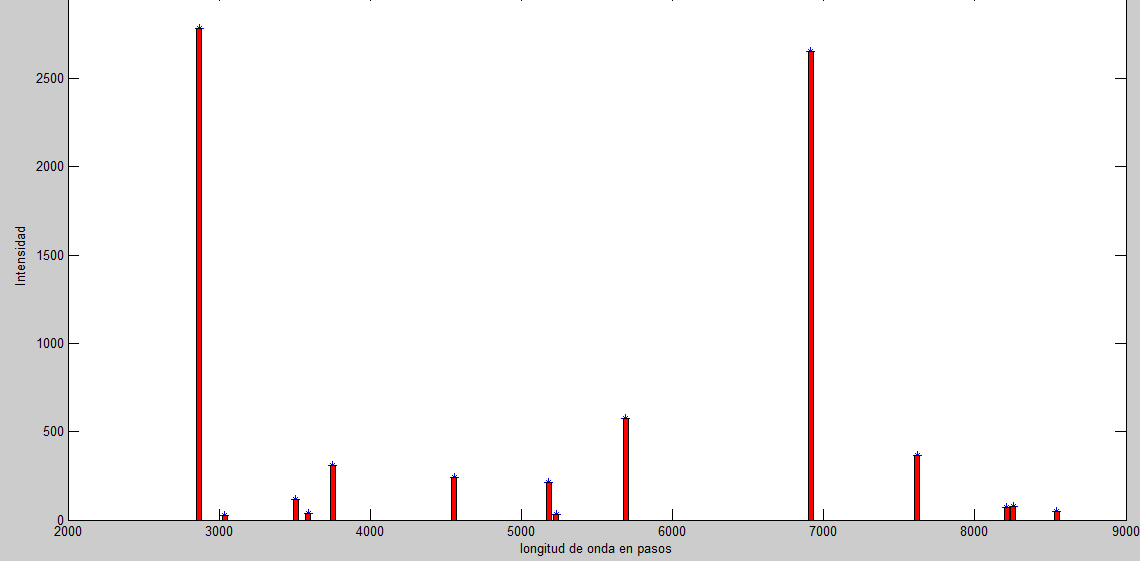
\includegraphics[width=0.9\linewidth, height=4.5cm]{Imagenes/3/picos14}
	
	\caption[Espectro de emisión de la lámpara de mercurio, espectro en intensidad contra pasos.]{Espectro de emisión de la lámpara de mercurio donde solo se grafica la posición y la intensidad de los 14 picos encontrados.}
	\label{fig:picos14}
\end{figure}

Con esta información se intenta encontrar cuánto varía un espectro del otro. En la figura \ref{fig:pasoserror} se puede apreciar la diferencia más grande en el paso, en el que se encuentra el pico es de 5 y de 3 la menor. %La desviación estándar del paso se ve en la figura \ref{fig:pasosdes}.

\begin{figure}[h]
	\centering
	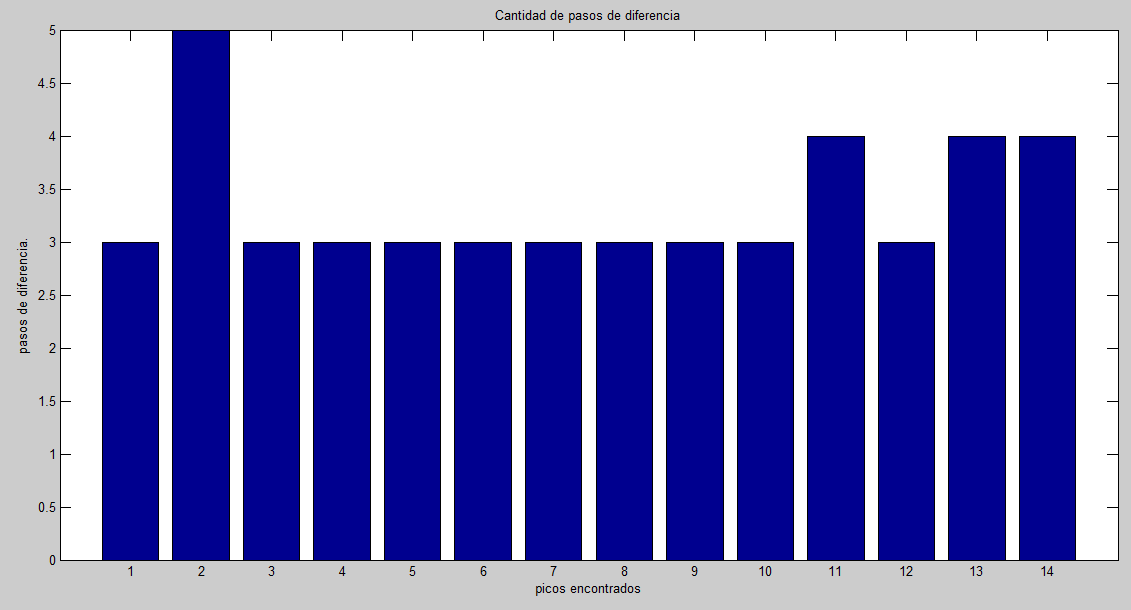
\includegraphics[width=0.8\linewidth,height=4cm]{Imagenes/3/pasosError}
	\caption[Diferencias de pasos en los picos encontrados.]{De los 14 picos encontrados se muestra la diferencia entre el paso en el que se encuentra cada pico. El máximo es de 5 pasos de diferencia y siendo 3 pasos lo normal.}
	\label{fig:pasoserror}
\end{figure}

 
%\begin{figure}[h]
%	\centering
%	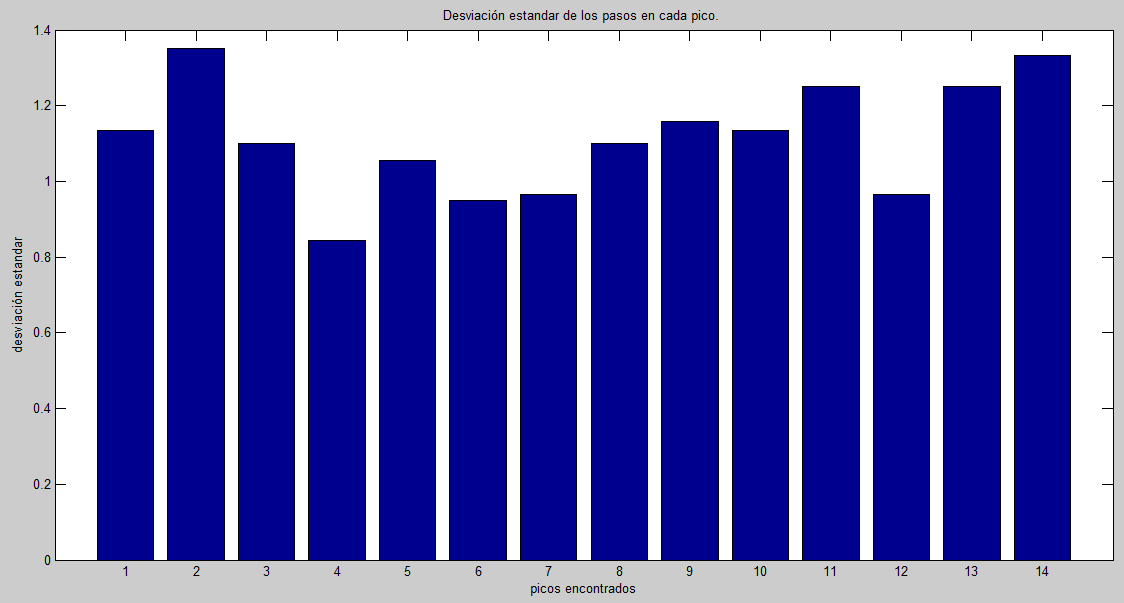
\includegraphics[width=0.8\linewidth,height=4cm]{Imagenes/3/pasosDes}
%	\caption{Desviación estándar de los pasos en los 14 picos encontrados.}
%	\label{fig:pasosdes}
%\end{figure}

La repetitividad del sistema es buena. Utilizando el promedio de las mediciones hechas se obtiene la relación paso longitud de onda. Al comparar el espectro medido con el sistema y el que se tiene en la literatura, se visualizan líneas de emisión  figura \ref{fig:espectroCompa}.
Para corroborar que varias de las líneas de emisión son de segundo orden se utilizó un filtro pasa alto mayor de 415nm. En la figura \ref{fig:hgfiltro} se aprecia como hay líneas de emisión que desaparecen al colocar el filtro. Con esta información se identifican las 12 líneas de emisión para la calibración.
\begin{figure}[h]
	\centering
	\subfigure[Espectro del Hg 12 líneas (no todas se ven en la gráfica.)]{	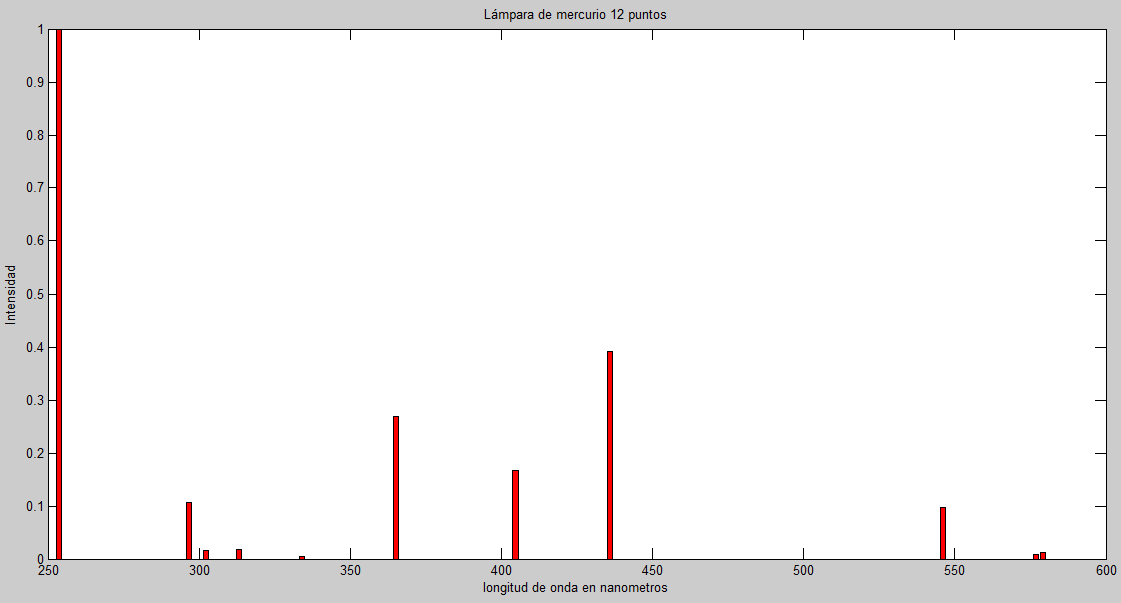
\includegraphics[width=0.45\linewidth, height=4cm]{Imagenes/3/espectroHgnor}}
	\subfigure[Espectro del Hg medido 14 líneas]{	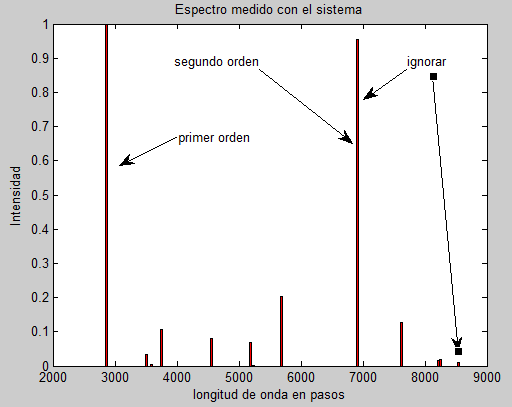
\includegraphics[width=0.45\linewidth, height=4cm]{Imagenes/3/espectroHgSistema}}
	\caption{Diferencia visible en la medición del espectro de la lámpara de mercurio. Hay dos líneas que no coinciden se decide cuales quitar.}
	\label{fig:espectroCompa}
\end{figure}
\begin{figure}[h]
	\centering
	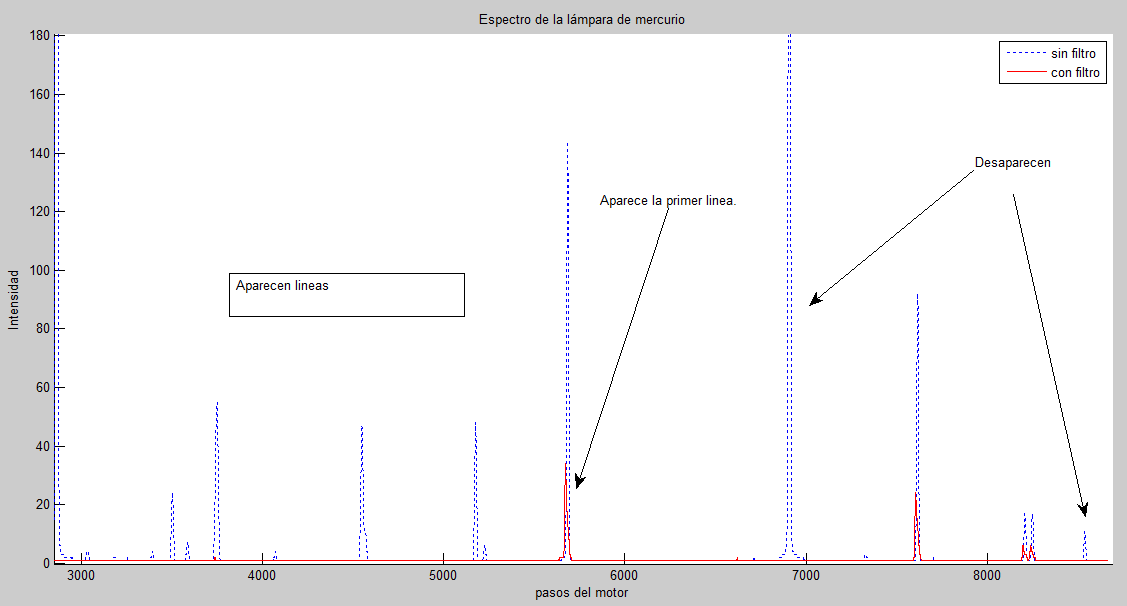
\includegraphics[width=0.75\linewidth, height=5cm]{Imagenes/3/HgFiltro}
	\caption[Espectro de la lámpara de mercurio con y sin filtro, intensidad contra pasos.]{Espectro de la lámpara de mercurio con y sin filtro, intensidad contra número de pasos. Se aprecia como la mayoría de las líneas desaparecen. Se prevé estas son menores a 415nm, y de las líneas de mayor longitud de onda solo desaparecen dos.}
	\label{fig:hgfiltro}
\end{figure}


%\begin{figure}
%	\centering
%	\subfigure[Espectro del Hg 12 líneas]{	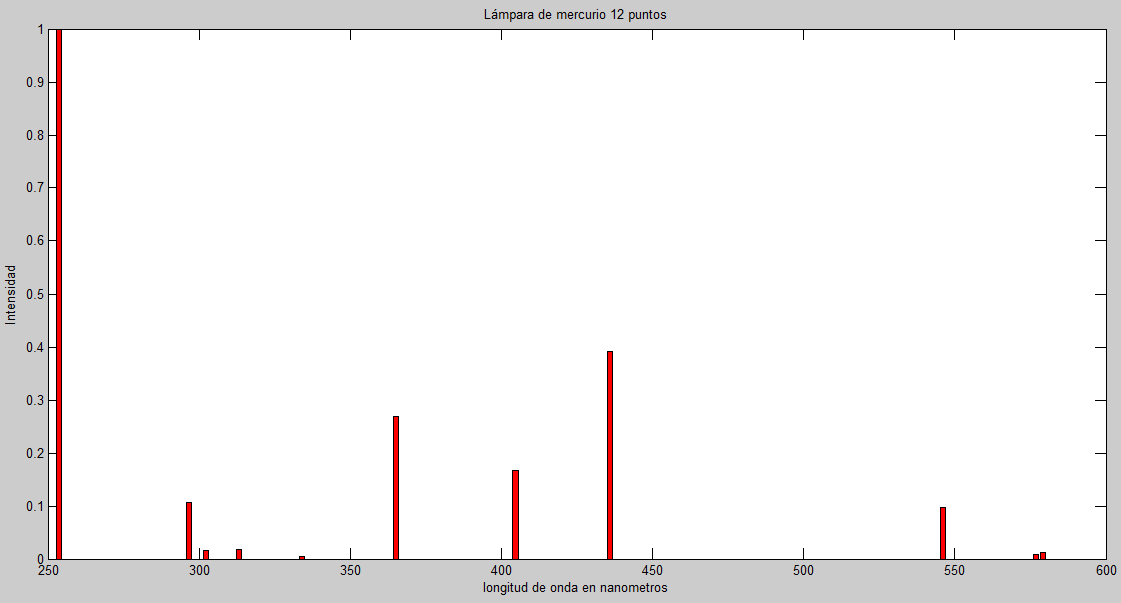
\includegraphics[width=0.4\linewidth]{Imagenes/3/espectroHgnor}}
%	\subfigure[Espectro del Hg medido 12 líneas]{	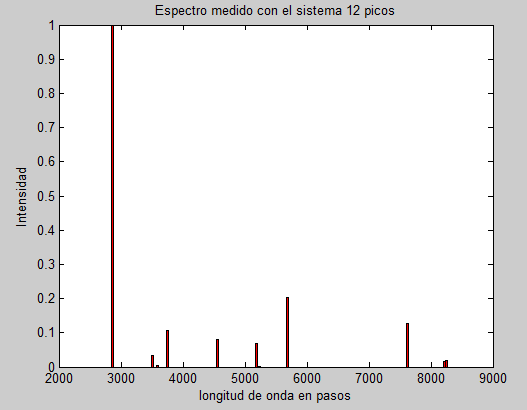
\includegraphics[width=0.4\linewidth]{Imagenes/3/espectroHgS12}}
%	\caption{Los espectros lucen visualmente muy similares, al quitar 2 de las líneas.}
%	\label{fig:espectroCom}
%\end{figure}

\subsubsection{Curve Fitting Tool.} 
El \textit{curve fitting} es un proceso para construir una función matemática, que se adapte a una serie de datos. Con este ajuste se tiene una interpolación. Lo que permite tener una relación paso a longitud de onda. Para obtener esta función se deben ingresar dos vectores a la herramienta. En la tabla \ref{tabla:pasolamda} se observan los datos que se utilizaron. El vector \textbf{Pasos} contiene los valores de los pasos en el que se encuentra cada pico. El vector \textbf{Lambda} son los valores de las líneas de emisión en nanómetros. La herramienta nos muestra los valores de "\textit{R-square} y \textit{RMSE}" para elegir la función con el mejor ajuste.
La figura \ref{fig:curving} es una captura de pantalla de la herramienta de \textbf{MATLAB}, \textbf{curve fitting tool}. 

\begin{table}[h]
	\caption{Las 12 líneas de emisión de la lámpara de mercurio, en nanómetros y el número de pasos que se encontró para cada una de estas líneas.}
	\label{tabla:pasolamda}
	\vspace{12mm}
	\begin{tabular}{|c|c|c|c|c|c|}
		\hline 
		Longitud de onda & Pasos & Longitud de onda & Pasos & Longitud de onda & Pasos \\ 
		\hline 
		253.652 & 2803 & 334.148 & 4011 & 435.833 & 5625 \\ 
		\hline 
		296.728 & 3442 & 365.015 & 4488 & 546.074 & 7558 \\ 
		\hline 
		302.150 & 3523 & 404.656 & 5116 & 576.96 & 8149 \\ 
		\hline 
		313.155 & 3690 & 407.783 & 5164 & 579.066 & 8190 \\ 
		\hline 
	\end{tabular} 
	
\end{table}

\begin{figure}[h]
	\centering
	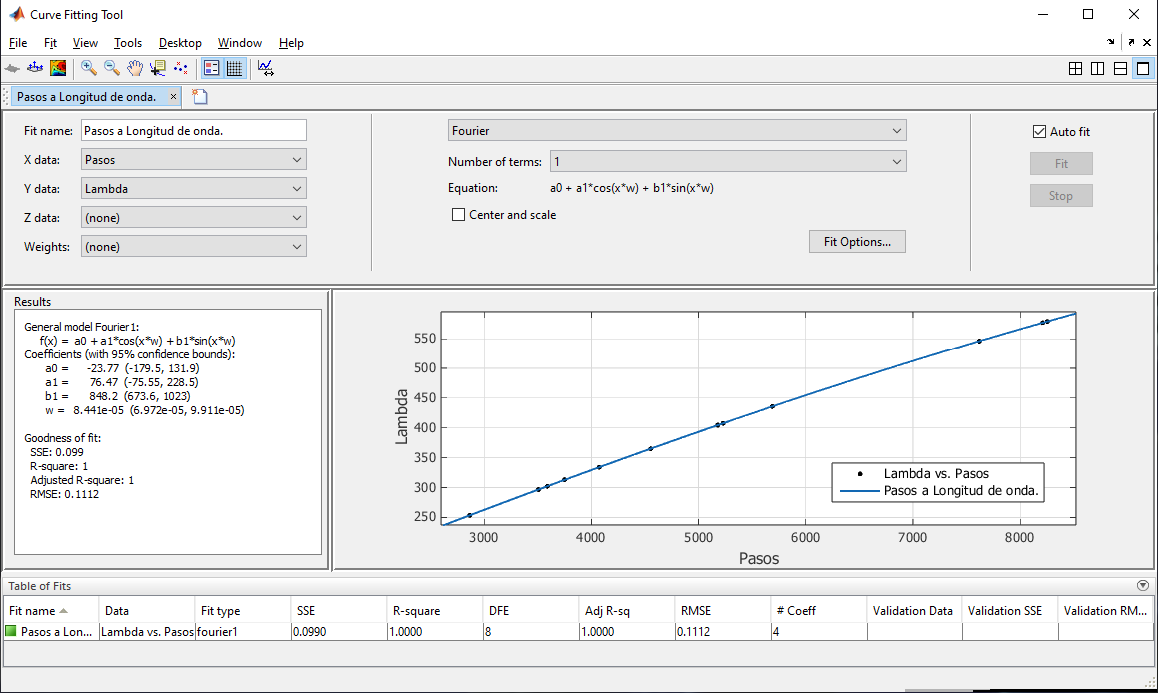
\includegraphics[width=1\linewidth,height=9cm]{Imagenes/3/curving}
	\caption{Interfaz de curve fitting tool de MATLAB.}
	\label{fig:curving}
\end{figure}
El coeficiente de determinación o también llamado $R^{2}$ o \textit{R-square}, en inglés. Es un valor que oscila entre 0 y 1. Entre más cerca este a 1 mayor será el ajuste del modelo a la variable que se está buscando. En general este valor es el más importante a la hora de buscar el mejor ajuste. EL RMSE, \textit{root-mean-square error} por sus siglas en inglés, es la raíz del error cuadrático medio, es una medida de uso frecuente de las diferencias entre los valores predichos por un modelo. Es una medida de precisión, para comparar errores de predicción de diferentes modelos. Su valor es siempre positivo y entre más cercano sea a cero menos es el error del ajuste.

En la tabla \ref{tabla:ajustes} se ve que varios ajustes tienen una \textit{$R^{2}$} igual a 1 pero con diferentes RMSE. El ajuste por Fourier con un solo término es el que tiene un RMSE = 0.1112.

 \begin{table} [h]
\centering
\caption{Diferentes ajustes obtenidos con \textit{curve fitting tool}. Varios de estos ajustes tienen una \textit{R-square} = 1. Por lo que se utiliza el siguiente criterio el RMSE. Siendo Fourier el mejor ajuste.}
\label{tabla:ajustes}
\begin{tabular}{|p{30mm}|p{30mm}|p{10mm}|p{12mm}|p{12mm}|p{12mm}|}
	\hline 
	Tipos de ajuste&Núm. de términos & $R^{2}$ & Adj $R^{2}$& RMSE & SSE \\ 
	\hline 
	Exponencial  & 1 & 0.9828 & 0.9811 & 15.5674 & 2423.4 \\ 
	\hline 
	& 2 & 1& 1 & 0.3485 & 0.9716 \\ 
	\hline 
	\textbf{Fourier} & 1 & 1 & 1 & 0.1112 & 0.0990 \\ 
	\hline 
	& 2 & 1 & 1 & 0.1283 & 0.0988 \\ 
	\hline 
	Gaussian & 3 & 1 & 1 & 0.1214 & 0.0442 \\ 	\hline 
	Polynomial & 3 & 1 & 1 & 0.1112 & 0.0989 \\ 
	\hline 
	Suma de senos & 1 & 1 & 1 & 0.3360 & 1.0161 \\ 
	\hline 
	& 3 & 1 & 1 & 0.1041 & 0.0325 \\ 
	\hline 
\end{tabular} 

\end{table}
La suma de senos con tres términos tiene mejores resultados, pero al intentar resolver la ecuación para obtener la relación opuesta, de longitud de onda a paso se encontraron problemas. Por lo anterior se trabajará con el ajuste de Fourier usando la ecuación \ref{equa:pasoLambda}.
\begin{equation}
f(x) = a_0 + a_1\cos (x\times w) + b_1 \sin(x \times w)
\label{equa:pasoLambda}
\end{equation}

Donde: \\
$x = pasos\\
a_0 =-23.77\\
a_1 = 76.47 \\  %(8.576, 247.4)
b_1 = 848.2 \\  %(774.8, 1030)
w = 8.441*10^{-5}$\\  %(7.044e-05, 8.994e-05)
La ecuación quedaría como:\\
\begin{equation}
f(x) =-23.77+76.47 \cos(pasos \times8.441\times10^{-5}) +848.2 \sin(pasos \times8.441\times10^{-5})
\label{equa:pasoLambda2}
\end{equation}

En la tabla \ref{tabla:comparaPasoL} se compara el espectro de emisión de la lámpara de mercurio contra la ecuación del ajuste. El error absoluto más grande es de $0.269$nm. En la figura \ref{fig:compararlp}, se aprecia el el espectro de la lámpara de mercurio medido con el sistema. Donde la relación ya es intensidad contra longitud de onda. Los asteriscos azules representan dónde deben aparecer las líneas de emisión. En rojo se aprecia el espectro medido.
   
\begin{table}[h]
	\centering 
	\caption{Comparación de la longitud de las líneas de emisión de la lámpara de mercurio y la ecuación obtenida para encontrar la relación de pasos a longitud de onda ($nm$).}
	\label{tabla:comparaPasoL}
	\begin{tabular}{|p{20mm}|p{20mm}|p{20mm}|p{20mm}|p{20mm}|p{20mm}|}
		\hline 
		 lámpara de Hg & Ajuste de paso a $\lambda$ & Diferencia  & lámpara de Hg & Ajuste de paso a $\lambda$ & Diferencia \\ 
		\hline 
		253.652 & 253.7412 & 0.0892 & 404.656 & 404.6091 & 0.0469 \\ 
		\hline 
		296.728 & 296.7452 & 0.0172 &407.783 & 407.7118 & 0.0712 \\ 
		\hline 
		302.15 & 302.1988 & 0.0488 &435.833 & 435.7680 & 0.065 \\ 
		\hline 
		313.155 & 312.9268 & 0.227 & 546.074 & 546.0847 & 0.0107  \\ 
		\hline 
		334.148 & 333.879 & 0.269 & 576.960 & 576.9355 & 0.0245  \\ 
		\hline 
		365.015 & 365.1355 & 0.1205 &  579.066 & 579.0719 & 0.0059\\ 
		\hline 
	\end{tabular} 
\end{table}

\begin{figure}[h]
	\centering
	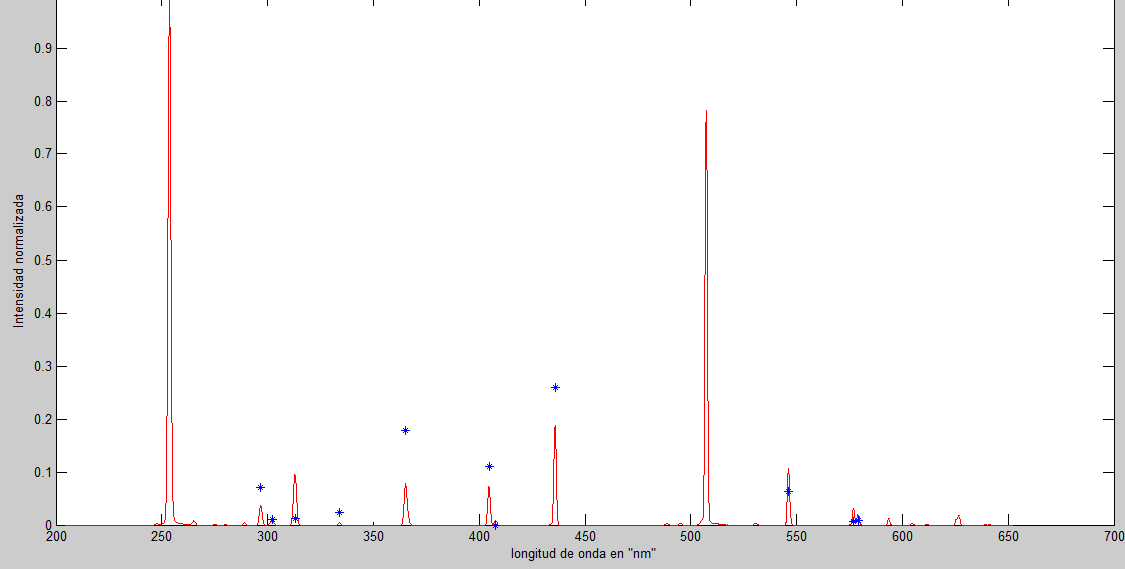
\includegraphics[width=1\linewidth,height=6.5cm]{Imagenes/3/compararLP}
	\caption{El espectro de emisión de la lámpara de mercurio, adquirido por nuestro sistema y ajustado con la ecuación, color rojo. El asterisco azul son las 12 líneas del espectro de emisión del mercurio. Se aprecia como coinciden estas 12 líneas con el espectro obtenido con el sistema.}
	\label{fig:compararlp}
\end{figure}
Este ajuste se introduce en la interfaz gráfica. De esta forma mientras se obtienen los datos, se visualiza el espectro medido, expresado en intensidad relativa contra longitud de onda. La figura \ref{fig:labviewmedir} es un ejemplo de medición con el sistema.\\
\begin{figure}[h]
	\centering
	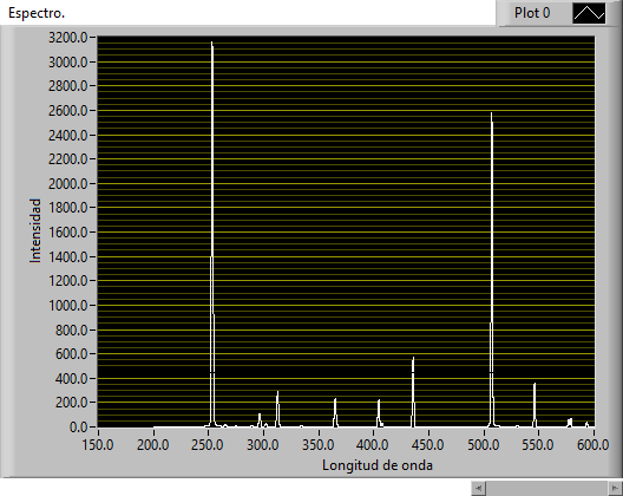
\includegraphics[width=0.9 \linewidth, height=6cm]{Imagenes/3/LabViewMedir}
	\caption{Espectro de la lámpara de mercurio medido con el sistema. La intensidad está en unidades relativas y la longitud de onda en nanómetros. El sistema ya está calibrado.}
	\label{fig:labviewmedir}
\end{figure}

\subsection{ADC MCP3202.}
%El ADC MCP3202 tiene una mayor resolución de 12 bits. 
En la figura \ref{fig:ledAmari}, se ve a la izquierda el espectro medido con el ADC del Arduino MEGA y a la derecha el ADC externo. 

\begin{figure}[h]
	\centering
	\subfigure[ADC propio del Arduino MEGA 10bits]{	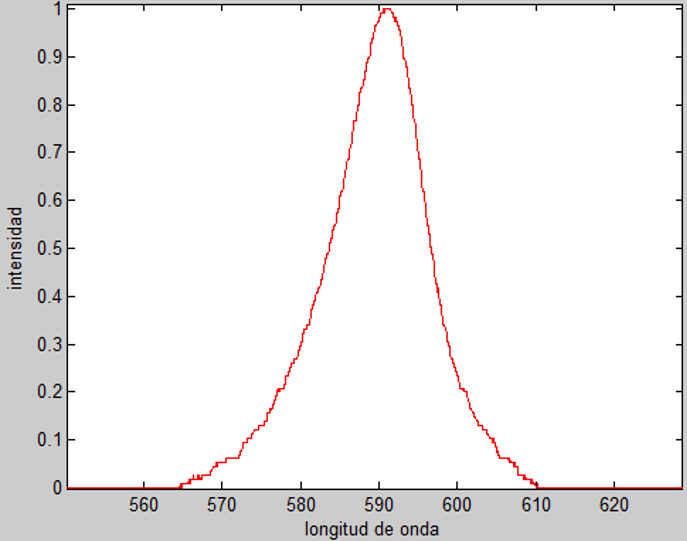
\includegraphics[width=0.48\linewidth,height=4cm]{Imagenes/3/LedAma10B}}
	\subfigure[ADC- MCP3202 de 12 bits]{	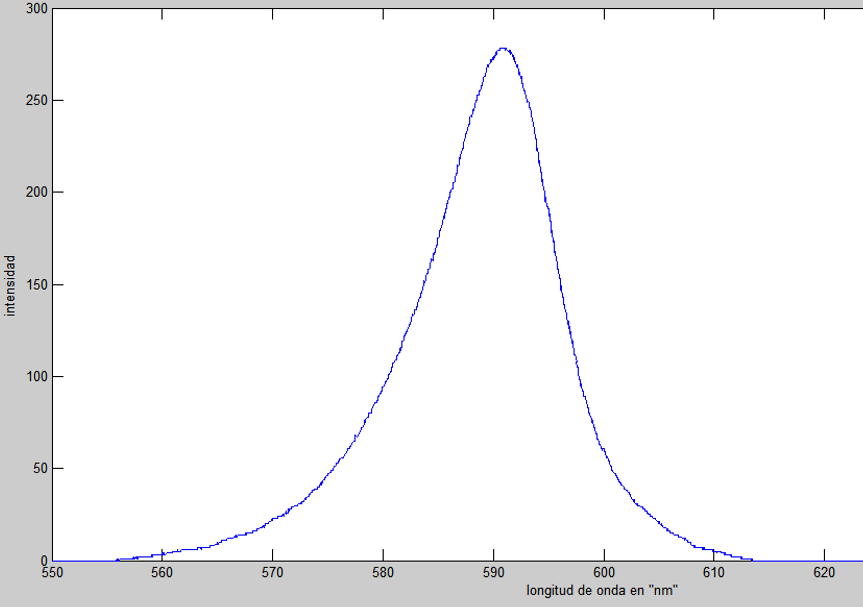
\includegraphics[width=0.48\linewidth,height=4cm]{Imagenes/3/LedAmaB12}}
	\caption{Comparación entre el ADC del Arduino MEGA, izquierda y el ADC MCP3202, derecha. Las dos gráficas están normalizadas.}
	\label{fig:ledAmari}
\end{figure}
El ADC MCP3202, es un ADC de 12 bits de resolución, el cual cuenta con comunicación serial SPI. 
Como se ha mencionado Arduino tiene una amplia comunidad, la cual día a día comparte trabajos y mejoras. Dentro de estos ya existen bibliotecas diseñadas para este ADC en específico. Una de ellas fue desarrollada por Souvik Saha \cite{MITadcLinkedIn}, su trabajo está en un repositorio de \textbf{GitHub}, \cite{MITadc} para que cualquier persona pueda usarlo así como en una página web dedicada a compartir bibliotecas, \cite{MITadcArduino}. Esta biblioteca fue ingresada en nuestro algoritmo.

\subsection{Potenciómetro digital.} 
La sensibilidad del \textbf{PMT} puede ser ajustada variando un voltaje de entrada en el módulo del \textbf{PMT}. Este ajuste se puede realizar de dos formas. Utilizando un potenciómetro o una fuente de voltaje variable ver figura \ref{fig:pmtsen}. Para este control se utilizó un potenciómetro digital. Así manipulamos el voltaje de control desde la interfaz gráfica.

\begin{figure}[h]
	\centering
	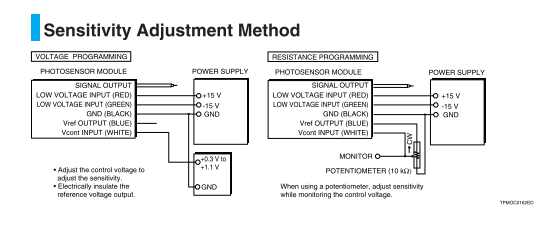
\includegraphics[width=0.9\linewidth]{Imagenes/3/PMTsen}
	\caption[Sensibilidad del \textit{PMT}.]{Esquema que muestra cómo modificar la sensibilidad del \textit{PMT}. Esta varía al cambiar el voltaje de control. Se puede realizar con una fuente variable o utilizando un potenciómetro y usando el voltaje de referencia del \textit{PMT}. \cite{H8249}}
	\label{fig:pmtsen}
\end{figure}
Se tomaron 10 valores de voltaje en cada paso del potenciómetro para ver cómo se comportaba y las variaciones de voltaje, ver figura \ref{fig:adcp1}(a). La figura \ref{fig:adcp1}(b) es la gráfica de la desviación estándar. Al hacer un acercamiento, véase figura \ref{fig:adcp1}(c), se aprecia que la desviación estándar es muy pequeña. En la figura \ref{fig:adcp1}(d) se observa el valor de las desviaciones estándar en cada paso. Siendo de 10mV el valor más grande de la desviación que es equivalente a un paso del potenciómetro digital. 

\begin{figure}[h!]
	\centering
	\subfigure[Voltaje en cada paso del potenciómetro digital.]{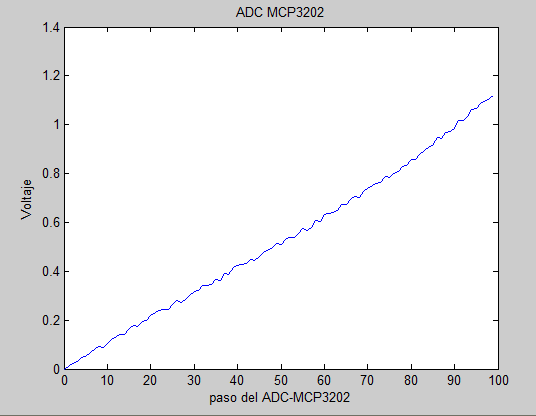
\includegraphics[width=0.48\linewidth,height=40mm]{Imagenes/3/ADCp1}}
%	\subfigure[promedio de 10 valores por paso]{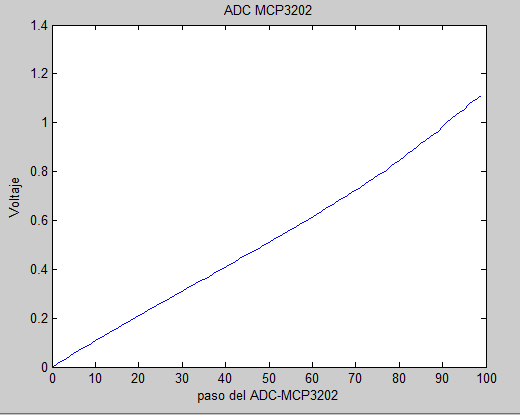
\includegraphics[width=0.48\linewidth,height=4cm]{Imagenes/3/ADCp1p}}
	\subfigure[Gráfica de la desviación estándar.]{\includegraphics[width=0.48\linewidth,height=40mm]{Imagenes/3/ADCpSTD}}
	\subfigure[desviación estándar de cerca. La variación de voltaje es de aproximadamente un paso, 10mV.]{\includegraphics[width=0.48\linewidth,height=40mm]{Imagenes/3/ADCpdifz}}
	\subfigure[Valor de la desviación estándar en cada paso.]{\includegraphics[width=0.48\linewidth,height=40mm]{Imagenes/3/ADCpdif}}
%	\subfigure[Grafica de la desviación estandar promedio de 10 valores por paso.]{\includegraphics[width=0.48\linewidth,height=4cm]{Imagenes/3/ADCpSTDp}}

%	\subfigure[error máximo 2.5mV]{\includegraphics[width=0.48\linewidth,height=4cm]{Imagenes/3/ADCpdifp}}
%	\subfigure[Error en porcentaje (0.91\%)]{\includegraphics[width=0.48\linewidth,height=4cm]{Imagenes/3/ADCpor}}
%	\subfigure[Error máximo 0.21\% ]{\includegraphics[width=0.48\linewidth,height=4cm]{Imagenes/3/ADCporp}}
	\caption[Comportamiento del potenciómetro digital X9C103]{Comportamiento del potenciómetro digital X9C103. Utilizando el voltaje de referencia del módulo de \textbf{PMT}. Se aprecia que la desviación estándar es muy pequeña. Así como las variaciones de voltaje, por lo que el sistema podrá medir de forma correcta.}
	\label{fig:adcp1}
\end{figure}
Al aumentar la sensibilidad del \textbf{PMT} se visualizan más líneas de emisión, y con mayor intensidad. Al realizar la medición con 0.2V, ya se aprecia el espectro de la lámpara de mercurio, ver figura \ref{fig:hglamp}(a). Al incrementar el voltaje que controla la sensibilidad del \textbf{PMT} a 0.5V. Se aprecia como en dos líneas de emisión, $\lambda$=253.6nm y en su segundo orden $\lambda$=507.2nm, el sistema se satura, véase figura \ref{fig:hglamp}(b).
\begin{figure}[h!]
	%\subfigure[Ganancia a 0.10 volts]{\includegraphics[width=0.48\linewidth,height=4cm]{Imagenes/3/Hg01}}
	\subfigure[Ganancia a 0.20 volts]{\includegraphics[width=0.48\linewidth,height=40mm]{Imagenes/3/Hg02}}
%	\subfigure[Ganancia a 0.30 volts]{\includegraphics[width=0.48\linewidth,height=35mm]{Imagenes/3/Hg03}}
%	\subfigure[Ganancia a 0.40 volts]{\includegraphics[width=0.48\linewidth,height=35mm]{Imagenes/3/Hg04}}
	\subfigure[Ganancia a 0.50 volts]{\includegraphics[width=0.48\linewidth,height=40mm]{Imagenes/3/Hg05}}
	\caption[Espectro de lámpara de mercurio medido con diferentes sensibilidades del \textbf{PMT}]{Espectro de lámpara de mercurio medido con diferentes sensibilidades del \textbf{PMT}. Al ir incrementando la sensibilidad del \textbf{PMT}, aumenta la intensidad captada en cada línea de emisión. Con lo que logramos observar más líneas.}
	\label{fig:hglamp}
\end{figure}
\newpage

\section{Intervalo espectral de trabajo del sistema. }
El PMT tiene un intervalo de sensibilidad que va desde los 180 nm hasta los 900 nm. Como se ve en la figura \ref{fig:respuesta}(a), su pico de sensibilidad está en los 400 nm, y a partir de aquí esta decae, al llegar a los 900 nm ya es mínima. Mientras que la red de difracción va desde los 200nm hasta los 850nm véase figura \ref{fig:respuesta}(b). Su máximo pico de eficiencia se encuentra en los 500nm aproximadamente, de aquí baja.
\begin{figure}[h]
	\centering
	\subfigure[Respuesta espectral del \textbf{PMT}, su pico de sensibilidad está en los 400nm]{\includegraphics[width=0.4\linewidth,height=4cm]{Imagenes/3/pmt_sen}}
	\subfigure[Eficiencia de la red de difracción con 2400 líneas/mm]{\includegraphics[width=0.4\linewidth,height=4cm]{Imagenes/3/redEfi}}
	\caption{Respuesta espectral de la red de difracción y del \textbf{PMT}, se aprecia que ambos empiezan en los 200nm, y llegan hasta los 800nm pero con sensibilidad mucho menos (\textbf{PMT}) \cite{H8249} y menor eficiencia (red de difracción. \cite{reddifrac})  }
	\label{fig:respuesta}
\end{figure}

Estos dos componentes serán los que limitarán el intervalo en el que nuestro sistema puede medir espectros. Se revisó el intervalo en el que puede trabajar el sistema, utilizando una lámpara de Tungsteno-Halógeno, de OceanOptics, esta lámpara tiene una respuesta espectral desde los 300 hasta los 1050 nm \cite{Manual1000}, figura \ref{fig:lamparathd}. Esta lámpara será más que suficiente para observar la sensibilidad del sistema a longitudes mayores a 600nm.\\
Al medir la lámpara LS-1-CAL, con el sistema desarrollado se tiene una gráfica con un valor máximo en la longitud de onda de 544.1nm, ver figura \ref{fig:lamparath}. Después de $lambda$=544.1nm la intensidad en el espectro decae hasta los 780nm. Esto se debe tanto al tubo fotomultiplicador como a la red de difracción como se explicó anteriormente.
\begin{figure}
	\centering
	\includegraphics[width=1\linewidth,height=6cm]{Imagenes/3/lamparaTH_DPNG}
	\caption{Espectro de la lámpara LS-1-CAL de OceanOptics. Usada para calibrar los espectrómetros en potencia. Su intervalo va desde los 300 nm hasta longitudes de onda mayores a los 1000nm. \cite{Manual1000}}
	\label{fig:lamparathd}
\end{figure}
\begin{figure}
	\centering
	\includegraphics[width=1\linewidth,height=6cm]{Imagenes/3/lamparaTH}
	\caption{Lámpara de tungsteno-halógeno de OceanOptics, LS-1-CAL. Medida con el sistema desarrollado. Se observa que el sistema comienza a decaer en sensibilidad a partir de los 540nm aproximadamente. Al llegar a los 780nm el sistema es incapaz de medir.}
	\label{fig:lamparath}
\end{figure}


